\documentclass[preprint,12pt]{elsarticle}
\usepackage{float}
\usepackage{placeins}
%% Use the option review to obtain double line spacing
%\documentclass[authoryear,preprint,review,12pt]{elsarticle}

%% Use the options 1p,twocolumn; 3p; 3p,twocolumn; 5p; or 5p,twocolumn
%% for a journal layout:
%% \documentclass[final,1p,times]{elsarticle}
%% \documentclass[final,1p,times,twocolumn]{elsarticle}
%% \documentclass[final,3p,times]{elsarticle}
%% \documentclass[final,3p,times,twocolumn]{elsarticle}
%% \documentclass[final,5p,times]{elsarticle}
%% \documentclass[final,5p,times,twocolumn]{elsarticle}

%% For including figures, graphicx.sty has been loaded in
%% elsarticle.cls. If you prefer to use the old commands
%% please give \usepackage{epsfig}
\usepackage[utf8]{inputenc}
\usepackage{comment}
\usepackage{lmodern}
\usepackage{textgreek}

%\usepackage[numbers,square]{natbib}
%% The amssymb package provides various useful mathematical symbols
\usepackage{amssymb}
%% The amsmath package provides various useful equation environments.
\usepackage{amsmath}
%% The amsthm package provides extended theorem environments
%% \usepackage{amsthm}

%% Pongo los números de línea porque lo pide la revista
\usepackage[left]{lineno}
\usepackage{listings}

\usepackage{hyperref}

\usepackage{booktabs}

\setlength{\marginparwidth}{2cm}

% Las figuras viven en paper/figures/ y las tablas generadas en eval/.
\graphicspath{{figures/}}

\sloppy

\journal{Automation in Construction}

\begin{document}
\linenumbers
\begin{frontmatter}

%% Title, authors and addresses

%% use the tnoteref command within \title for footnotes;
%% use the tnotetext command for theassociated footnote;
%% use the fnref command within \author or \affiliation for footnotes;
%% use the fntext command for theassociated footnote;
%% use the corref command within \author for corresponding author footnotes;
%% use the cortext command for theassociated footnote;
%% use the ead command for the email address,
%% and the form \ead[url] for the home page:
\title{A Systematic Comparative Study of Retrieval Methods for Parametric Construction Catalogs: From Lexical to Neural Approaches}

\author[deptA,b]{Cesáreo González-Alvarez\corref{cor1}}
\cortext[cor1]{Corresponding author}
\ead{cgonza06@estudiantes.unileon.es}
%% \ead[url]{home page}

\author[deptA]{Laura Fernández-Robles}
\author[deptA]{Enrique Alegre}
\author[deptA]{Manuel Castejón-Limas}

\affiliation[deptA]{organization={Group for Vision and Intelligent Systems, I4 Institute, Universidad de León},
%%             addressline={},
               city={León},
               postcode={24071},
%%             state={},
               country={Spain}}
\affiliation[b]{organization={Telice S.A.},
            city={[León]},
            postcode={[24391]},
            country={Spain}}               

%% Abstract
\begin{abstract}

Construction projects increasingly rely on large parametric catalogs containing tens
of thousands of near-identical items, where accurate retrieval is critical for cost
estimation and procurement. This paper presents a systematic comparison of lexical,
neural, and hybrid information retrieval methods for matching short work descriptions
against a large-scale parametric catalog of Spanish railway infrastructure. The
catalog's hierarchical structure enables a dual evaluation at item level (exact
variant) and parent level (family). Across 100 configurations evaluated on
approximately 47,500 catalog items, a tuned BM25 with domain-specific parameter
phrases achieves 97.4% top-1 accuracy, outperforming the best neural retriever
(BGE-M3-ColBERT, 44.8%) by over 52 percentage points and all hybrid configurations by
more than 8 points. Neural embeddings remain competitive at the parent level (up to
99.7%) but fail to discriminate fine-grained variants; roughly 98% of errors involve
numeric parameters. Well-tuned lexical retrieval thus provides a strong, interpretable
baseline for parametric construction catalog search.

\end{abstract}

%% Keywords
\begin{keyword}
%% keywords here, in the form: keyword \sep keyword
%% PACS codes here, in the form: \PACS code \sep code
%% MSC codes here, in the form: \MSC code \sep code
%% or \MSC[2008] code \sep code (2000 is the default)
Information retrieval \ Construction catalog \ BM25 \ Dense retrieval \ Parametric catalog \ Benchmark dataset
\end{keyword}

\end{frontmatter}

\section*{Glossary}

\begin{description}

    \item[Acc@1] Accuracy at rank 1 --- the proportion of queries for which the correct item appears in the top position.
 
    \item[ADIF] Spanish acronym for \textit{Administrador de Infraestructuras Ferroviarias}, the public entity responsible for railway infrastructure in Spain.

    \item[BC3 Format] Base de Costes de la Construcción, version 3 --- the standard data exchange format for Spanish construction cost databases, encoding hierarchical cost structures with parametric templates and work item descriptions.

    \item[BM25] A probabilistic ranking function that scores document relevance based on term frequency and document length normalization.

    \item[Dense Retrieval] A neural retrieval approach that represents queries and documents as dense embeddings, enabling semantic similarity search via vector spaces.

    \item[E5 Model] A sentence-transformer-based embedding model trained for general-purpose retrieval and semantic similarity tasks.
    
    \item[Hard-Negative Retrieval] A retrieval scenario where the correct item must be distinguished from highly similar candidates differing only in one or more critical attributes, such as a numeric specification.

    \item[Hybrid Retrieval] A method that combines lexical and neural approaches, often through score fusion or reranking, to balance precision and semantic coverage.

    \item[Item-Level / Parent-Level Evaluation] A dual evaluation protocol assessing retrieval at two granularities: item-level requires retrieving the exact parametric variant, while parent-level credits any item from the same parametric family.
    
    \item[Language Model (LM)] A lexical retrieval method that estimates the probability of generating a query from a document's language distribution.
    
    \item[MRR] Mean Reciprocal Rank — the average reciprocal of the rank position of the first relevant result across all queries.
    
    \item[nDCG] Normalized Discounted Cumulative Gain --- a ranking metric that accounts for graded relevance and result position.

    \item[Parametric Catalog] A structured database where construction items are described by sets of parameters.  Each unique combination of parameter values generates a distinct catalog item.
    
    \item[Pseudo-Relevance Feedback (PRF)] A technique that expands the query using top-ranked documents from an initial retrieval round to improve recall.

\end{description}

\section{Introduction}
In modern construction project management, accurately retrieving the correct work item from standardized catalogs  is critical for budget control, procurement and stakeholder communication ~\cite{martinez-rojasApproachAutomaticClassification2015, natural_wu_2022}. Large infrastructure projects increasingly rely on parametric construction catalogs containing tens of thousands of highly similar items, where small lexical or numeric differences correspond to distinct technical specifications and unit costs. In this context, catalog retrieval is a precision-critical task rather than a general semantic search problem.

The challenge is compounded by terminology variability across stakeholders. Field workers, designers, and cost estimators often use different terms for identical concepts, creating a vocabulary mismatch between queries and catalog entries  ~\cite{chungComparingNaturalLanguage2023, role_martnezrojas_2016, rampiniArtificialIntelligenceConstruction2022, casiniAdvancedSiteManagement2022}. Moreover, construction descriptions frequently contain critical numeric parameters—dimensions, quantities, specifications—where even minor discrepancies can lead to costly errors in project estimation ~\cite{natural_wu_2022}. These domain-specific characteristics demand retrieval methods that balance lexical precision with semantic understanding while maintaining sensitivity to numeric values.

These terminology mismatches are particularly evident in two operational contexts. First, during cost estimation for design-bid-build tenders, estimators must map project specifications—often drafted with company-specific or region-specific wording—to standardized catalog entries. A project item description related to pipes must be matched to the precise catalog variant that accounts for terrain type, pipe diameter, and work-shift conditions, yet the source document may omit or paraphrase critical parameters. Second, during project execution, field engineers produce daily progress reports using abbreviated or colloquial item descriptions that must be reconciled with contractual line items for billing and compliance. A site note should map unambiguously to a specific catalog entry, but the terse phrasing and implicit context challenge both manual lookup and automated systems. In both scenarios, failure to retrieve the correct item carries tangible consequences: cost overruns from misquoted unit prices, contractual disputes over scope interpretation, or delays in payment certification. Robust retrieval methods that tolerate terminological variation while preserving numeric and parametric precision are therefore essential to practical construction workflows.

Attempts to automate this mapping process predominantly employed rule-based systems and traditional machine learning methods, which often rely on structured data sets and expert-driven input ~\cite{caldasAutomatingHierarchicalDocument2003, natural_wu_2022}. Although these methods have shown limited success, they struggle with the domain-specific variability, nuanced language, and unstructured data prevalent in construction management ~\cite{rampiniArtificialIntelligenceConstruction2022, baekCriticalReviewTextbased2021}. Advances in natural language processing (NLP), particularly transformer-based models such as BERT, have shown promise in addressing these challenges by capturing semantic variability and contextual relationships ~\cite{tangAutomatedConstructionQuantity2022, dezaMachineLearningApproach2022}. However, issues such as data sparsity, domain-specific jargon, and computational resource demands persist ~\cite{chungComparingNaturalLanguage2023, martinez-rojasUsingClassificationTechniques2018}.

This study addresses these challenges through a systematic comparative evaluation of lexical, neural and hybrid retrieval methods for a large-scale construction catalog in the railway infrastructure domain. Using short-format catalog descriptions as queries and long-format entries as retrieval targets, we simulate realistic scenarios in which descriptions are shortened, paraphrased, or reformulated. The task is to retrieve the exact matching item among nearly forty thousand candidates from a single parametric subcategory, a setting where small lexical or numeric differences can determine success or failure.

This study addresses these challenges through a systematic comparative evaluation of lexical, neural and hybrid retrieval methods for a large-scale construction catalog in the railway infrastructure domain. Using short-format catalog descriptions as queries and long-format entries as retrieval targets, we simulate realistic scenarios in which descriptions are shortened, paraphrased, or reformulated. The task is to retrieve the exact matching item among nearly forty thousand candidates from a single parametric subcategory, a setting where small lexical or numeric differences can determine success or failure.

Figure~\ref{fig:retrieval_workflow} summarizes the retrieval setting considered in this study, from short catalog descriptions, used as proxies for practitioner-oriented queries, to the identification of the corresponding detailed construction item.

\begin{figure}[H]
    \centering
    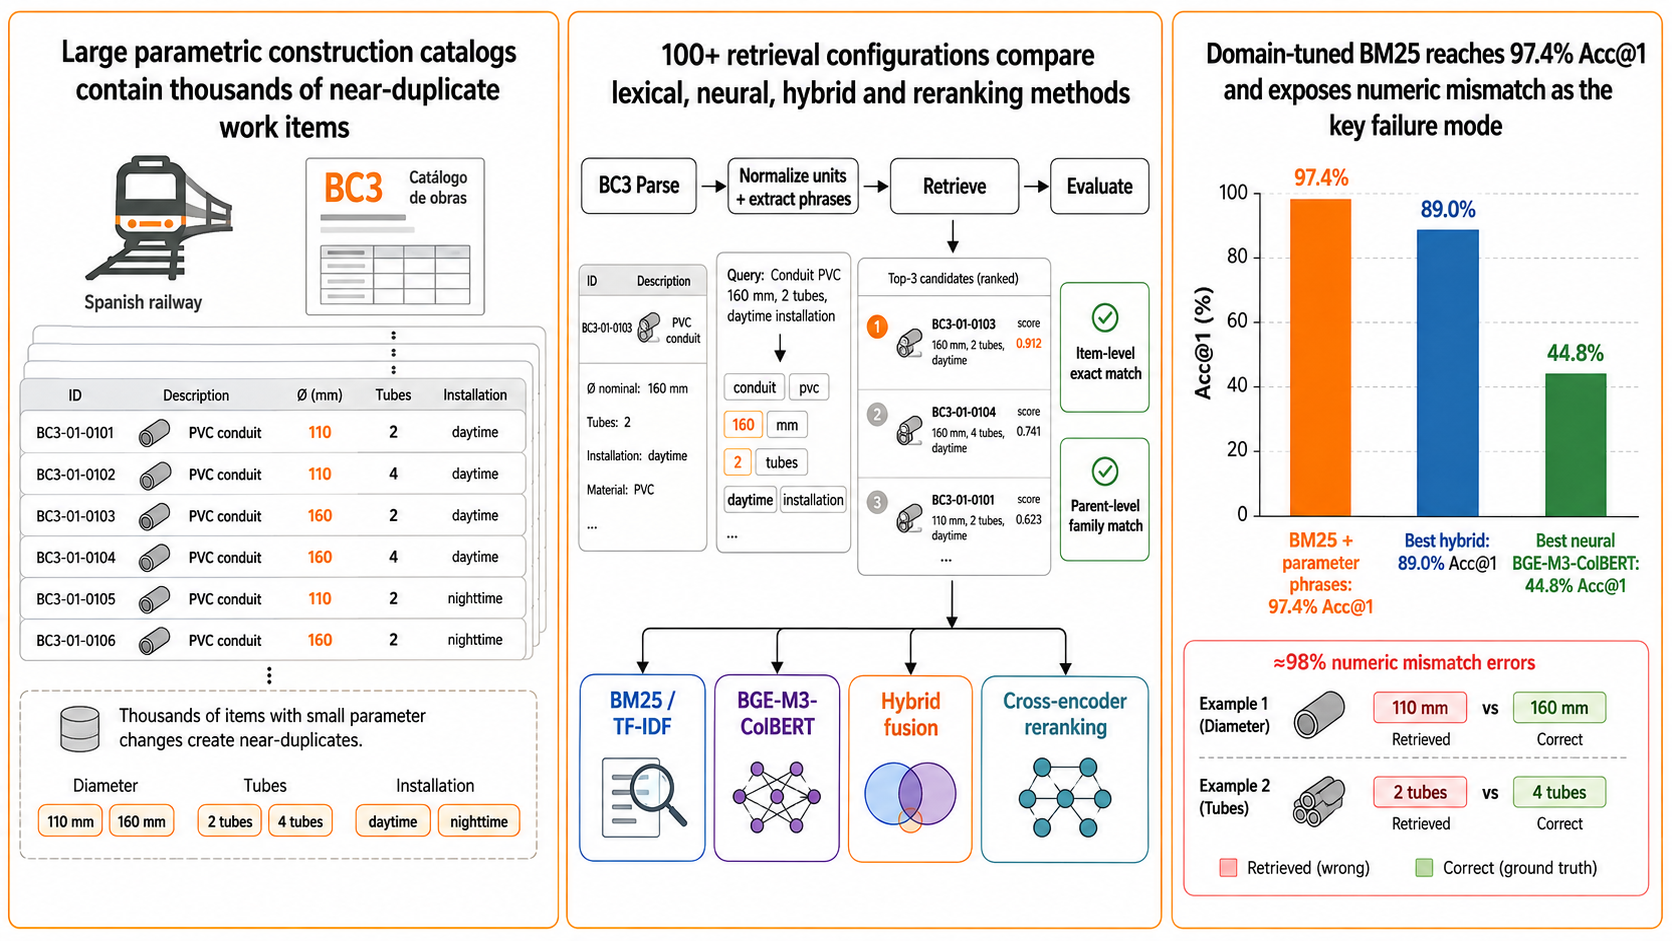
\includegraphics[width=\linewidth]{graphical_abstract.png}
    \caption{Overview of the construction catalog retrieval task evaluated in this study. Short catalog descriptions are used as proxy practitioner-oriented queries to retrieve the exact matching item from a large parametric catalog, where near-duplicate entries may differ only in technical or numeric attributes.}
    \label{fig:retrieval_workflow}
\end{figure}

Our contributions are fourfold:

\begin{itemize}
    \item We present a systematic comparison of lexical, sparse, dense, and hybrid retrieval methods, including pseudo-relevance feedback and cross-encoder reranking, in a precision-critical technical domain.
    \item We introduce an evaluation protocol that incorporates multiple metrics, dual target definitions (item- and parent-level), and significance testing, ensuring a rigorous and reproducible assessment.
    \item We conduct detailed error analysis, identifying numeric mismatches and near-duplicate confusions as dominant error modes, thus offering insights for future research on retrieval in structured domains.
    \item We create and release a structured benchmark dataset derived from the OEB subcategory of ADIF's parametric railway catalog — a homogeneous yet challenging testbed of nearly 40,000 items exhibiting high parametric variability — including custom parsing tools to convert the raw BC3 catalog format into a standardized retrieval evaluation dataset ~\cite{bc3cat_dataset}.
    
\end{itemize}

The rest of this paper is organized as follows: Section 2 reviews prior work on construction classification and retrieval methods. Section 3 describes the ADIF dataset, preprocessing pipeline, and the $100$ retrieval configurations evaluated. Section 4 presents results showing that optimized lexical methods consistently outperform neural and hybrid approaches at the item level, while neural models remain competitive at the parent level. Section 5 discusses the implications of these findings for construction catalog deployment, and Section 6 concludes with directions for future research. 

\section{Prior Work}

\subsection{Construction Classification Systems and Standards}

Construction work breakdown structures present a fundamental taxonomic challenge that distinguishes this domain from general information retrieval applications. National and organizational classification systems—including MasterFormat, UniFormat, OmniClass, and infrastructure-specific frameworks such as the ADIF (Spanish National Railway Manager) railway catalog \href{https://bpa.adif.es/bp1/#/welcome}{ADIF´s BPA Catalog} used in this study—impose hierarchical structures where items are organized by trade, material, location, or function ~\cite{royanoAnalysisClassificationSystems2023a, guvenConstructionClassificationSystem2022}. These parametric catalogs contain thousands to tens of thousands of work items characterized by structured attributes (dimensions, materials, performance specifications, unit costs) alongside free-text descriptions that exhibit substantial terminological variability. The ADIF catalog examined here, for instance, contains approximately 47,500 distinct work items spanning civil works, track infrastructure, electrification, and signaling systems.

The vocabulary mismatch problem is particularly acute in construction contexts. Practitioners use regional terminology, abbreviations, brand names, and informal descriptors that diverge significantly from standardized catalog entries. A single concept—such as a reinforced concrete beam of specific dimensions—may appear under dozens of lexical variants across project documents, specifications, and bills of quantities. This heterogeneity is further compounded in multilingual settings and when integrating catalogs from different organizations. 

Prior work has addressed this complexity through ontology-based approaches. The Industry Foundation Classes (IFC) and International Framework for Dictionaries (IFD) provide semantic frameworks for mapping between classification systems and enabling interoperability across software platforms. ~\cite{wuNaturallanguagebasedIntelligentRetrieval2019} developed natural-language retrieval engines for BIM object databases using vector-space models enhanced with domain ontologies, establishing a paradigm where lexical retrieval is augmented with explicit semantic expansion. ~\cite{43f8dc68b3d05e73df8185c5a051e207a64e4ed4} proposed Enhanced Explicit Semantic Analysis for construction product model retrieval, leveraging concept spaces derived from construction knowledge bases to bridge vocabulary gaps. ~\cite{wangMultiscaleInformationRetrieval2021} extended this work with multi-scale BIM information retrieval using hierarchical structure modeling based on IFC. These foundational approaches established that effective retrieval in construction requires explicit handling of domain semantics, though they predate the neural revolution in information retrieval and have not been systematically compared against modern dense retrieval methods.

\subsection{Automated Classification and Retrieval in Construction}

The application of natural language processing and machine learning to construction document processing has grown substantially over the past decade. Early work by ~\cite{caldasAutomatingHierarchicalDocument2003} applied text classification to organize construction project documents, while subsequent studies extended these methods to bills of quantities, specifications, and regulatory texts. Systematic reviews by ~\cite{wuNaturalLanguageProcessing2022} and ~\cite{chungComparingNaturalLanguage2023} document the evolution from rule-based and bag-of-words approaches through support vector machines to contemporary transformer-based methods.

Most published work in construction NLP addresses category-level classification rather than item-level retrieval. ~\cite{tangAutomatedConstructionQuantity2022} applied deep learning to construction specification classification; ~\cite{martinez-rojasUsingClassificationTechniques2018} developed automated text classification pipelines for public procurement documents using support vector machines and later neural approaches. Jacques de Sousa et al. recently reviewed automation approaches for the budgeting phase, finding that text classification methods achieve reasonable accuracy for category assignment but struggle with fine-grained item matching.

Critically, classification accuracy degrades as taxonomic granularity increases. ~\cite{caldasAutomatingHierarchicalDocument2003} reported 95.88\% accuracy for top-level MasterFormat divisions but substantially lower performance for fine-grained subcategories. Similarly, ~\cite{martinez-rojasApproachAutomaticClassification2015} achieved 92.4\% accuracy at the chapter level of work breakdown structures, with performance declining for detailed categorization. ~\cite{dezaMachineLearningApproach2022} explored bidirectional LSTMs and Temporal Convolutional Networks for short construction text classification, demonstrating that even modern sequence models struggle with the brevity and density of catalog-style descriptions. These findings underscore that the granularity required for item-level retrieval—distinguishing among tens of thousands of near-identical entries—exceeds the capabilities demonstrated in existing classification studies.

\subsection{Technical Catalog Retrieval: Methods and Cross-Domain Evidence}

Information retrieval for technical catalogs has received extensive attention in e-commerce and manufacturing domains, offering methodological insights transferable to construction applications. The fundamental architectural choice—lexical versus neural retrieval—has been systematically evaluated in product search contexts with findings directly relevant to parametric construction catalogs.

Lexical methods, exemplified by BM25 and its variants, remain remarkably competitive for technical domains. ~\cite{mendesComparativeStudyLexical2025} compared BM25 against semantic embedding methods on governmental product catalogs and electronic invoices, finding that lexical retrieval achieved faster identification of relevant products while semantic methods improved ranking within retrieved sets. This complementarity motivates hybrid architectures. ~\cite{changExtremeMultilabelLearning2021} demonstrated that sparse TF-IDF representations with extreme multi-label classification (the PECOS framework) achieved superior recall and latency on catalogs exceeding 100 million items compared to dense neural embeddings trained on the same data. ~\cite{ubrangalaSearchingFastSlow2024} showed that character-level TF-IDF outperformed word-level variants for SKU search with abbreviation-heavy queries—a finding directly applicable to construction catalogs where alphanumeric codes and abbreviated specifications are prevalent. These results suggest that technical identifiers, part numbers, and precise parametric specifications benefit from exact matching that dense representations may inadvertently blur.

Neural approaches have nonetheless advanced substantially in product retrieval. Dual-encoder architectures trained on large-scale click logs demonstrate strong performance when vocabulary mismatch is substantial and paraphrase recognition is required. ~\cite{nigamSemanticProductSearch2019a} at Amazon introduced semantic product search using bi-encoder transformers, achieving significant improvements in recall over lexical baselines. ~\cite{choiSemanticProductSearch2020} developed structured matching modules that encode multi-field product information—titles, descriptions, dimensions, metadata—into unified representations that respect the heterogeneous structure of catalog entries. The CHARM architecture ~\cite{freymuthHierarchicalMultifieldRepresentations2025} proposed cascading hierarchical attention to align query tokens with specific product fields. More recent work explores learned sparse retrieval, where neural networks generate interpretable term expansions that combine lexical precision with semantic generalization. ~\cite{biswasEfficientInterpretableInformation2024} showed that hybrid encoders jointly learning dense and sparse representations can match cross-encoder effectiveness while maintaining first-stage retrieval efficiency—a critical consideration for production systems with latency constraints.

Relevant cross-domain work also addresses procurement and product standardization. The TPDR system ~\cite{cunhaTPDRNovelTwoStep2023} developed for intermediary procurement—including construction-related purchases—employs a two-stage architecture: dual transformer encoders for initial retrieval followed by syntactic reranking. This hybrid approach achieved substantial gains over purely lexical or purely semantic baselines when matching noisy, abbreviated initial specifications to standardized product descriptions. Cross-lingual product matching systems using hierarchical metric learning ~\cite{kooDeepMetricLearning2023} further demonstrate how taxonomy-aware training objectives can distinguish exact duplicates from substitutes and unrelated items—a distinction critical for construction catalogs where material grades or dimensional variants carry significant cost implications.

\subsection{Research Gap and Contribution}

Despite the maturity of retrieval methods in adjacent domains, no systematic benchmark exists for evaluating lexical, neural, and hybrid approaches on construction parametric catalogs. The AEC-specific literature remains dominated by ontology-enhanced lexical methods developed before the transformer era, with limited adoption of the dense retrieval and learned sparse techniques that have transformed e-commerce search. Meanwhile, the product search literature, while methodologically sophisticated, lacks evaluation on the particular characteristics of construction work items: dense parametric specifications with numeric constraints, deep hierarchical classification structures, and domain-specific terminology in languages beyond English. This gap leaves practitioners without empirical guidance when selecting retrieval architectures for construction applications.

This study addresses that gap through a systematic comparison of retrieval methods on a large-scale Spanish railway construction catalog. We evaluate classical lexical baselines (BM25 with domain-specific preprocessing including Spanish stemming and stopword handling), neural dense retrievers (multilingual sentence transformers fine-tuned for semantic similarity), and hybrid configurations that combine lexical and neural signals. Our experimental design encompasses 100 retrieval configurations across realistic query scenarios reflecting practitioner search behavior. The findings provide empirical guidance for practitioners implementing catalog retrieval systems and contribute the first rigorous benchmark for information retrieval on parametric construction work items, demonstrating conditions under which carefully tuned lexical methods remain competitive with—or superior to—neural alternatives.

\section{Methodology}

\subsection{Dataset Characteristics and Processing}

\subsubsection{Dataset Scope and Selection}

The experimental dataset derives from ADIF's parametric price catalog for Spanish railway infrastructure. While the complete catalog spans ten technical chapters (Architecture, Civil Works, Control Systems, Energy, Environmental Management, Protection and Security, Safety and Health, Telecommunications, and Track), this study focuses on the OEB subcategory within the Civil Works chapter, which addresses platform system infrastructure such as trenches, conduits, and piping systems, providing a controlled yet demanding testbed for retrieval evaluation. Extending the benchmark to additional chapters remains a priority for future work, as discussed in Section~\ref{sec:discussion}.

The OEB subcategory provides an ideal testbed for retrieval evaluation as it exhibits high parametric variability while maintaining manageable scope for comprehensive analysis. Through parametric expansion of base templates across combinations of pipe materials, diameters (110mm, 160mm, 200mm), quantities (2, 4, 6, 8, 12 tubes), terrain types (normal, rocky, under tracks, road crossing, platform, attached, ballast), and work shift specifications (daytime, nighttime, exceptional conditions), the subcategory generates 47513 distinct item variants ~\cite{bc3cat_dataset}.

Each of these item variants belongs to a hierarchical structure:  
- The \emph{item-level} contains the fully specified variant, including all parameters (e.g., “6 PVC tubes, 160mm, under tracks, nighttime”).  
- The \emph{parent-level} refers to the shared base template that groups multiple such variants under a common parametric definition.

Table~\ref{tab:dataset_statistics} presents key characteristics of the processed dataset.

\begin{table}[ht]
\centering
\caption{OEB Subcategory Dataset Statistics}
\label{tab:dataset_statistics}
\begin{tabular}{|l|r|}
\hline
\textbf{Characteristic} & \textbf{Value} \\
\hline
Total unique items & 47,513 \\
Base templates & 30 \\
Average expansion factor & 1583.8 \\
\hline
\textit{Short-Format description (`resumen')} (query) & \\
\quad Mean length (words) & 19.7 \\
\quad Median length (words) & 20 \\
\quad Std deviation (words) & 2.4 \\
\hline
\textit{Long-Format description (`texto')} (target) & \\
\quad Mean length (words) & 84.5 \\
\quad Median length (words) & 83 \\
\quad Std deviation (words) & 15.0 \\
\hline
Queries with numeric parameters & 47,430 (99\%) \\
Queries without numeric parameters & 83 (0\%) \\
Single-item templates ($=$1 variants) & 25 (0\%) \\
\hline
\end{tabular}
\end{table}
\smallskip
\small\textit{Note:} `resumen' and `texto' are the field names in the original Spanish dataset.
\smallskip

To illustrate the dataset structure, Figure \ref{fig:oeb_example} presents a translated example from the original Spanish corpus. A template (e.g., OEB020\$) defines a base construction concept and several configurable parameters. Each unique combination of parameter values produces a distinct item, with both a concise short-format description used as the query and a detailed long-format description serving as the retrieval target.

\begin{figure}[ht]
\centering
\small
\fbox{\parbox{0.92\textwidth}{
\textbf{Template:} OEB020\$ — Concrete-encased PVC conduit, 110 mm\\[6pt]
%
\textbf{Parameters:}\\
\begin{tabular}{@{}ll@{}}
No. of pipes & 2 \\
Terrain type & Normal \\
Work shift & Daytime \\
Maintenance window & $\geq$5 hours \\
Execution conditions & High volume \\
\end{tabular}\\[6pt]
%
\textbf{Short-format (\textit{resumen}):}\\
Concrete-encased conduit, 2 pipes, PVC 110 mm, normal terrain. (Daytime / i $\geq$5h / High volume)\\[6pt]
%
\textbf{Long-format (\textit{texto}):}\\
Concrete-encased conduit installation of 2 PVC pipes, 110 mm diameter, in any terrain except rock, including trench backfilling and compaction, supply and installation of pipes and HE-20 concrete (non-vibrated), conduit testing, transport and removal of materials to worksite. Work shift: Daytime. Maintenance window: $\geq$5 hours. Execution conditions: High volume.
}}
\caption{Example item from the OEB dataset (translated from Spanish). Each template expands into multiple items by varying parameter combinations.}
\label{fig:oeb_example}
\end{figure}

\subsubsection{BC3 Format Processing}

ADIF distributes its catalog in BC3 format (Base de Costes de la Construcción), the standard exchange format established by FIEBDC, a Spanish industry consortium that maintains data interchange standards for construction cost databases. We developed a custom parsing pipeline to transform the BC3 specification into structured JSON suitable for retrieval experiments.

The parsing pipeline handles three key transformations:

\begin{enumerate}
    \item \textbf{Parametric Expansion}: The BC3 format encodes base items with parameter placeholders (e.g., \texttt{\textbackslash No\_PIPES\textbackslash}, \texttt{\textbackslash TERRAIN\_TYPE\textbackslash}). The parser extracts parameter definitions, generates all valid combinations, and instantiates complete item descriptions by substituting parameter values into templates.
    
    \item \textbf{Dual-Text Extraction}: Each item contains two text fields: \textit{short-format} (condensed summary with parametric codes) and \textit{long-format} (detailed technical specification). The parser extracts both fields while preserving their association through unique item identifiers.
    
    \item \textbf{Metadata Preservation}: The parser retains hierarchical information including chapter codes, base template identifiers (first 6 characters), and parametric family relationships to enable parent-level evaluation.
\end{enumerate}

The complete parsing pipeline implementation is available in our code repository ~\cite{bc3cat_software}.

\subsubsection{Text Preprocessing}

All text fields undergo standardized preprocessing before indexing and retrieval. The preprocessing pipeline applies the following transformations:

\paragraph{Normalization}
\begin{itemize}
    \item Lowercase conversion for case-insensitive matching
    \item Whitespace standardization (multiple spaces → single space)
    \item Punctuation preservation except for sentence-final periods
    \item Numeric normalization (e.g., ``1,256.84'' for ``1256,84'')
    \item Accented character retention for proper Spanish processing
\end{itemize}

\paragraph{Tokenization}
Different retrieval methods receive appropriately tokenized input:
\begin{itemize}
    \item \textbf{Word tokens}: Regex pattern \texttt{\textbackslash w+} for lexical methods, yielding sequences like \texttt{["conduit", "concrete-cased", "2", "pipes", "pvc", "110", "mm"]}
    \item \textbf{Character n-grams}: Overlapping sequences of length 3, 4, and 5 for character-based methods (e.g., ``pvc'' → \texttt{["pvc", "\#pv", "pvc", "vc\#"]})
    \item \textbf{Subword tokens}: Pretrained tokenizers for neural methods (WordPiece for BERT-based models, SentencePiece for others)
\end{itemize}

\paragraph{Parameter-Based Phrase Identification}
We leverage the catalog's parametric structure to identify domain-specific multi-word expressions. From the BC3 parameter definitions, we extract 127 multi-word parameter values (e.g., terrain types, work conditions, installation contexts) that function as atomic units in the classification system.

The preprocessing pipeline evaluated two phrase handling strategies:
\begin{itemize}
    \item \textbf{Additive}: Phrases supplement unigrams (``road'', ``crossing'', ``road\_crossing'')
    \item \textbf{Replacement}: Phrases substitute component words (``road\_crossing'' only)
\end{itemize}

This domain-specific phrase handling enables retrieval methods to align with the catalog's inherent parametric vocabulary.

\paragraph{Numeric Feature Extraction}
The pipeline identifies and normalizes integer quantities, decimal measurements with units, numeric ranges, and percentages.

Extracted numeric features enable exact numeric matching as a complementary retrieval signal (Section~\ref{subsec:hybrid_fusion}).

\subsection{Retrieval System Configurations}

We evaluate 100 distinct retrieval configurations organized into four method families. Table~\ref{tab:method_families} summarizes the configuration space.

\begin{table}[ht]
\centering
\caption{Overview of Evaluated Retrieval Configurations}
\label{tab:method_families}
\begin{tabular}{|l|r|p{6cm}|}
\hline
\textbf{Method Family} & \textbf{Configs} & \textbf{Key Variations} \\
\hline
Lexical (BM25 \& TF-IDF) & 67 & Parameter tuning, tokenization, phrase handling \\
Pseudo-Relevance Feedback & 16 & RM3 and Rocchio with various feedback parameters \\
Neural Dense Retrieval & 7 & E5, GTE, BGE-M3 models with different settings \\
Hybrid \& Reranking & 10 & Fusion methods and cross-encoder reranking \\
\hline
\textbf{Total} & \textbf{100} & \\
\hline
\end{tabular}
\end{table}

\subsubsection{Lexical Methods: BM25 and TF-IDF}
\label{subsec:lexical_methods}

\paragraph{BM25 Implementation}

We implement BM25 using Pyserini v0.21.0~\citep{lin2021pyserini}, which provides efficient indexing and retrieval through the Lucene backend. We evaluate three tokenization variants, each with its own parameter grid:
\begin{itemize}
    \item \textbf{BM25-unigram}: Standard word tokenization\\
    $k_1 \in \{0.6, 0.8, 1.0, 1.2, 1.4\}$, $b \in \{0.20, 0.35, 0.50, 0.65, 0.80\}$ (25 combinations)
    \item \textbf{BM25-unibigram}: Word unigrams + bigrams\\
    $k_1 \in \{0.8, 1.0, 1.2, 1.4, 1.6\}$, $b \in \{0.35, 0.50, 0.65, 0.80, 0.95\}$ (25 combinations)
    \item \textbf{BM25-unigram-params}: Word tokens + parameter-derived phrases\\
    $k_1 \in \{0.6, 0.8, 1.0, 1.2\}$, $b \in \{0.35, 0.50, 0.65\}$ (12 combinations)
\end{itemize}

This yields 62 total configurations. Documents and queries undergo identical preprocessing before indexing. Index construction uses default Lucene analyzers with custom stopword lists removed (domain-specific terms like ``of'', ``in'' carry meaning in construction context).

\paragraph{TF-IDF Implementation}
TF-IDF baselines use scikit-learn v1.2.2~\citep{pedregosa2011scikit} with the following configurations:
\begin{itemize}
    \item \textbf{TF-IDF-unigram}: Word unigrams with standard stopword removal
    \item \textbf{TF-IDF-unigram-nonstop}: Word unigrams without stopword removal
    \item \textbf{TF-IDF-char}: Character n-grams ($n \in \{3,4,5\}$) with word boundary markers
    \item \textbf{TF-IDF-phrases-add}: Word unigrams augmented with parameter-derived phrase tokens (e.g., ``High volume'')
    \item \textbf{TF-IDF-phrases-replace}: Multi-word parameter phrases replaced by single tokens
\end{itemize}
All TF-IDF variants use cosine similarity for ranking with L2-normalized vectors.

\subsubsection{Pseudo-Relevance Feedback Methods}

We evaluate two PRF methods using the same parameter grid: feedback documents $M \in \{5, 10\}$, expansion terms $N \in \{20, 40\}$, and feedback weight $\beta \in \{0.5, 0.7\}$, yielding 8 configurations each (the two weakest β=0.7, N=40 variants are
omitted for brevity; full results in the repository).

\paragraph{RM3} It uses Pyserini's built-in PRF module with BM25 as the base retriever, where $\beta$ controls interpolation between the original query and the relevance model.

\paragraph{Rocchio} It uses scikit-learn with TF-IDF representations, where $\beta$ weights the feedback centroid. No negative feedback is used ($\gamma = 0$) due to the single-relevant-item setting.

\subsubsection{Neural Dense Retrieval Methods}

All neural models are used in zero-shot mode without fine-tuning on construction text, testing their transfer capabilities to domain-specific Spanish technical language.

\paragraph{E5 Model}
We evaluate \texttt{intfloat/multilingual-e5-base} (278M parameters, 768 dimensions) using the sentence-transformers library v2.2.2~\citep{reimers2019sentence}. Following the model documentation, queries receive the prefix ``query: '' and documents receive ``passage: '' before encoding. Embeddings are L2-normalized before similarity computation.

\paragraph{Spanish Sentence Similarity}
We evaluate \texttt{hiiamsid/sentence\_similarity\_spanish\_es}, a model specifically fine-tuned for Spanish semantic similarity tasks, to compare against multilingual alternatives.

\paragraph{GTE Model}
We evaluate \texttt{Alibaba-NLP/gte-multilingual-base} with two query formats:
\begin{itemize}
    \item \textbf{GTE-direct}: Standard ``query:'' prefix
    \item \textbf{GTE-instruct}: Spanish instruction prefix: ``query: Lookup for the most similar document to this query: [query]''
\end{itemize}

\paragraph{BGE-M3 Model}
BGE-M3 (\texttt{BAAI/bge-m3}, 568M parameters) supports three retrieval modes within a unified architecture~\citep{chen2024bge}:
\begin{itemize}
    \item \textbf{BGE-M3-dense}: Single 1024-dimensional vector per text
    \item \textbf{BGE-M3-sparse}: Learned sparse weights (SPLADE-style)
    \item \textbf{BGE-M3-colbert}: Token-level embeddings with ColBERT-style late interaction
\end{itemize}
The ColBERT mode computes relevance as the sum of maximum token similarities. All BGE-M3 modes use the same encoder with mode-specific output layers.

\subsubsection{Hybrid Fusion and Reranking}
\label{subsec:hybrid_fusion}

The fusion process consisted of three sequential steps applied to each query independently.

First, retrieval scores from each ranker were normalized using min-max scaling to ensure comparability across heterogeneous scoring functions. For a given query $q$, document $d$ and ranker $r$, each document score $s_{d,r}$ was transformed as:

\begin{equation}
s'_{d,r} = \frac{s_{d,r} - \min_r(s)}{\max_r(s) - \min_r(s)}
\end{equation}

Second, we applied numeric parameter bonuses to account for matches between query parameters and document metadata. Each document received an additional weighted reward based on exact parameter matches ($\beta_{\text{exact}}$) and partial parameter overlaps ($\beta_{\text{overlap}}$). These bonuses were added to the normalized scores before fusion.

Third, the adjusted scores from all retrievers were combined using weighted linear combination (COMBSUM):

\begin{equation}
s_{\text{final}}(d) = \sum_{r \in R} w_r \cdot s'_{d,r}
\end{equation}

where $w_r$ represents the fusion weight for ranker $r$, and $\sum_{r} w_r = 1$.

To identify optimal fusion configurations, we conducted a systematic parameter sweep over the weight space for several hybrid strategies: (1) three-way fusions combining BM25 with one BGE-M3 variant and character-level TF-IDF, and (2) a five-way fusion incorporating BM25, all three BGE-M3 variants (dense, sparse, ColBERT), and TF-IDF. For each configuration, we evaluated combinations of $\beta_{\text{exact}} \in \{0.0, 0.05, 0.1\}$ and $\beta_{\text{overlap}} \in \{0.0, 0.05\}$ across a grid of weight distributions. The optimal configuration for each strategy was selected based on MRR@10 performance on the test set.

\paragraph{Cross-Encoder Reranking}
We employ a two-stage cascade: efficient first-stage retrieval followed by expensive cross-encoder reranking of top candidates. Cross-encoder implementation uses:

\begin{itemize}
    \item Model: \texttt{cross-encoder/ms-marco-MiniLM-L-6-v2} (22M parameters)
    \item Input format: \texttt{[CLS] query [SEP] document [SEP]}
    \item Reranking depth: Top 20, 50, or 100 candidates from first stage
    \item Base retrievers: BM25, E5-large, and hybrid configurations
\end{itemize}

The cross-encoder produces a relevance score for each query-document pair through joint encoding and classification head. We evaluate the performance gain versus computational cost across different reranking depths.

\subsection{Evaluation Protocol}

\subsubsection{Retrieval Task Definition}

The evaluation task simulates realistic construction catalog search: given a short-form description (\textit{resumen}), retrieve the corresponding detailed specification (\textit{texto}) from 47,513 candidates. Each query has exactly one correct target at the item level, though multiple items may share the same parametric parent.

We construct the evaluation set by:
\begin{enumerate}
    \item A random sample of 16,590 from the \textit{resumen} descriptions was selected as query inputs
    \item All 47,513 \textit{texto} descriptions were used as the retrieval corpus
    \item Ground truth mappings were defined using shared item identifiers
    \item The full catalog was retained as distractors-no filtering or candidate pruning was applied
\end{enumerate}

The sample size (16,590) ensures 99\% confidence with ±1\% margin of error:
\[
n = \frac{Z^2 \cdot p(1 - p)}{E^2} = \frac{(2.576)^2 \cdot 0.5 \cdot 0.5}{(0.01)^2} = 16{,}590
\]
where $n$ is the required sample size, $Z$ is the Z-score for the confidence level (2.576 for 99\%), $p = 0.5$ assumes maximum variance, and $E$ is the margin of error (0.01). This ensures statistically robust comparisons across methods.

\subsubsection{Dual-Target Evaluation}

We implement two complementary evaluation perspectives:

\paragraph{Item-Level (Exact Match)}
Requires retrieving the specific parametric variant. For query with ID ``OEB020aabdcfa'', only the document with identical ID counts as correct. This strict criterion applies to scenarios requiring precise specifications such as material procurement or detailed cost estimation.

\paragraph{Parent-Level (Family Match)}
Credits retrieval of any variant from the same parametric family, identified through shared 6-character prefixes. For query ``OEB020aabdcfa'', any document with ID starting ``OEB020'' counts as correct. This relaxed criterion acknowledges scenarios where parametric siblings are functionally equivalent, such as preliminary estimation or category identification.

The dual-target approach enables nuanced analysis: methods may excel at family identification while struggling with variant-level disambiguation.

\subsubsection{Evaluation Metrics}

We employ five complementary metrics to assess retrieval quality:

\begin{enumerate}
    \item \textbf{Accuracy@1 (Success@1)}: Proportion of queries where the correct item appears in rank 1. Critical for automated systems where only the top result is used.
    
    \item \textbf{Recall@k}: Proportion of queries with correct item in top-$k$ results. We report Recall@5 and Recall@10 as reasonable examination depths for human review.
    
    \item \textbf{Mean Reciprocal Rank (MRR)}: Average of reciprocal ranks of first correct result.
    
    \item \textbf{Normalized Discounted Cumulative Gain (nDCG@10)}: Accounts for rank position using logarithmic discount
    
    \item \textbf{Mean Average Precision (MAP)}: Averaged precision at each relevant result.
\end{enumerate}

All metrics are computed using the ranx library v0.3.7~\citep{bassani2022ranx}, which provides efficient implementations with built-in significance testing.

\subsubsection{Query Subset Analysis}

Performance analysis across query subsets reveals how methods handle different retrieval challenges. We partition the evaluation set into two categories:

\begin{itemize}
    \item \textbf{HAS\_NUM} (24,711 queries, 62\%): Queries containing at least one numeric parameter (e.g., ``2 tubos'', ``110 mm''). Tests whether methods can match quantitative specifications.
    
    \item \textbf{NO\_NUM} (15,136 queries, 38\%): Queries without numeric content, containing only textual descriptors. Isolates purely textual matching performance.

\end{itemize}

Subset analysis identifies method strengths (e.g., neural models may excel on NO\_NUM while lexical methods dominate HAS\_NUM).

\subsubsection{Statistical Significance Testing}

We employ paired bootstrap resampling to determine whether observed performance differences reflect genuine method advantages rather than random variation~\citep{smucker2007comparison}.

For each system pair $(A, B)$, we compute per-query metric differences, generate $B=10{,}000$ bootstrap samples with replacement, and estimate $p$-values from the empirical distribution of mean differences. We apply Bonferroni correction for multiple comparisons and report improvements as significant only when $p < 0.05$ after correction.

\subsubsection{Error Analysis}

To understand failure modes, we analyze 100 randomly sampled errors from each method family. Errors are categorized into:

\begin{enumerate}
    \item \textbf{Numeric Mismatch}: Retrieved item differs from target in quantitative parameters (e.g., ``110 mm'' vs ``160 mm'', ``2 tubos'' vs ``4 tubos'')
    
    \item \textbf{Lexical Confusion}: High lexical overlap masks critical distinctions, particularly in work condition modifiers (e.g., standard vs exceptional shifts) or scope descriptors (e.g., supply-only vs supply-and-installation)
    
    \item \textbf{Near-Duplicate Error}: Correct item exists but parametric sibling ranks higher due to high lexical similarity
    
    \item \textbf{Ranking Failure}: Correct item retrieved but ranks beyond typical examination depth (position 11+)
\end{enumerate}

Error distribution reveals systematic failure patterns that guide method selection for different deployment contexts.

\subsection{Implementation Details}

All experiments use Python 3.10 with Pyserini for BM25/RM3, scikit-learn for TF-IDF/Rocchio, sentence-transformers and FlagEmbedding for neural models, and ranx for evaluation~\citep{bassani2022ranx}. Experiments run on servers with Intel i9-13900KF CPUs and 4× NVIDIA RTX 4090 GPUs. For reproducibility, random seeds are fixed, model versions pinned, and complete configurations stored in YAML files; code and data are openly available at ~\cite{bc3cat_software,bc3cat_dataset}. 

\section{Results}
The results across all evaluated configurations converge on a consistent finding: lexical methods, when properly tuned with domain-specific parameter phrases, outperform neural and hybrid approaches at the item level by a substantial margin. The following subsections detail the performance of each method family, culminating in a cross-method comparison in Section~\ref{sec:4.7_Overall Performance Summary}.

\subsection{Lexical Methods Comparative Analysis}

The performance of all lexical retrieval configurations was evaluated at two hierarchical levels: parent-level and item-level retrieval. Figure~\ref{fig:lexical_performance_parent} presents parent-level results, where the task is to retrieve the correct parent document, while Figure~\ref{fig:lexical_performance_item} shows item-level results for retrieving specific document items. Both evaluations used the same test set of 16,590 queries.

At the parent level (Figure~\ref{fig:lexical_performance_parent}), TF-IDF methods dominated, with TF-IDF-unigram\_phrases\_replace achieving the highest Acc@1 (0.990). BM25 variants showed more modest parent-level performance, ranging from 0.873 to 0.985.

\begin{figure}[htbt]
\centering
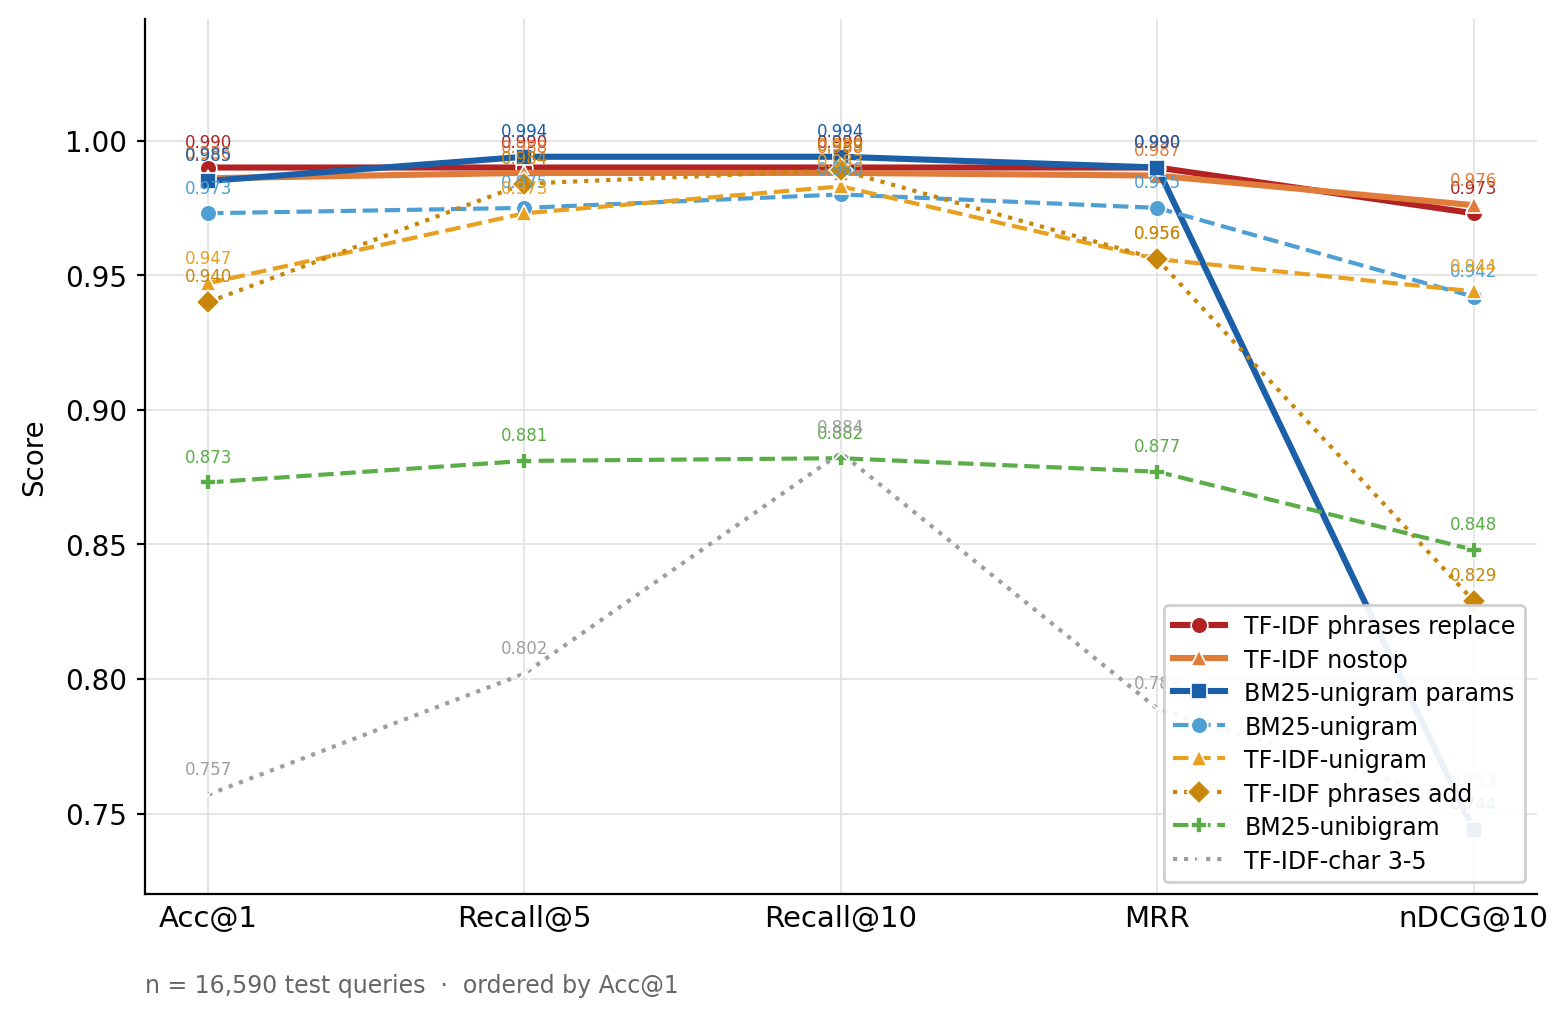
\includegraphics[width=\textwidth]{lexical_performance_parent.png}
\caption{Performance comparison of lexical retrieval methods at parent level on the test set (n=16,590 queries). Methods are ranked by Accuracy@1.}
\label{fig:lexical_performance_parent}
\end{figure}

At the item level (Figure~\ref{fig:lexical_performance_item}), the ranking inverted. BM25-unigram\_params achieved the highest Acc@1 (0.974), while TF-IDF methods dropped substantially (0.558--0.708). This $26.6$ percentage point gap between the best BM25 and best TF-IDF demonstrates that document-length normalization is critical for fine-grained catalog discrimination.

\begin{figure}[htbt]
\centering
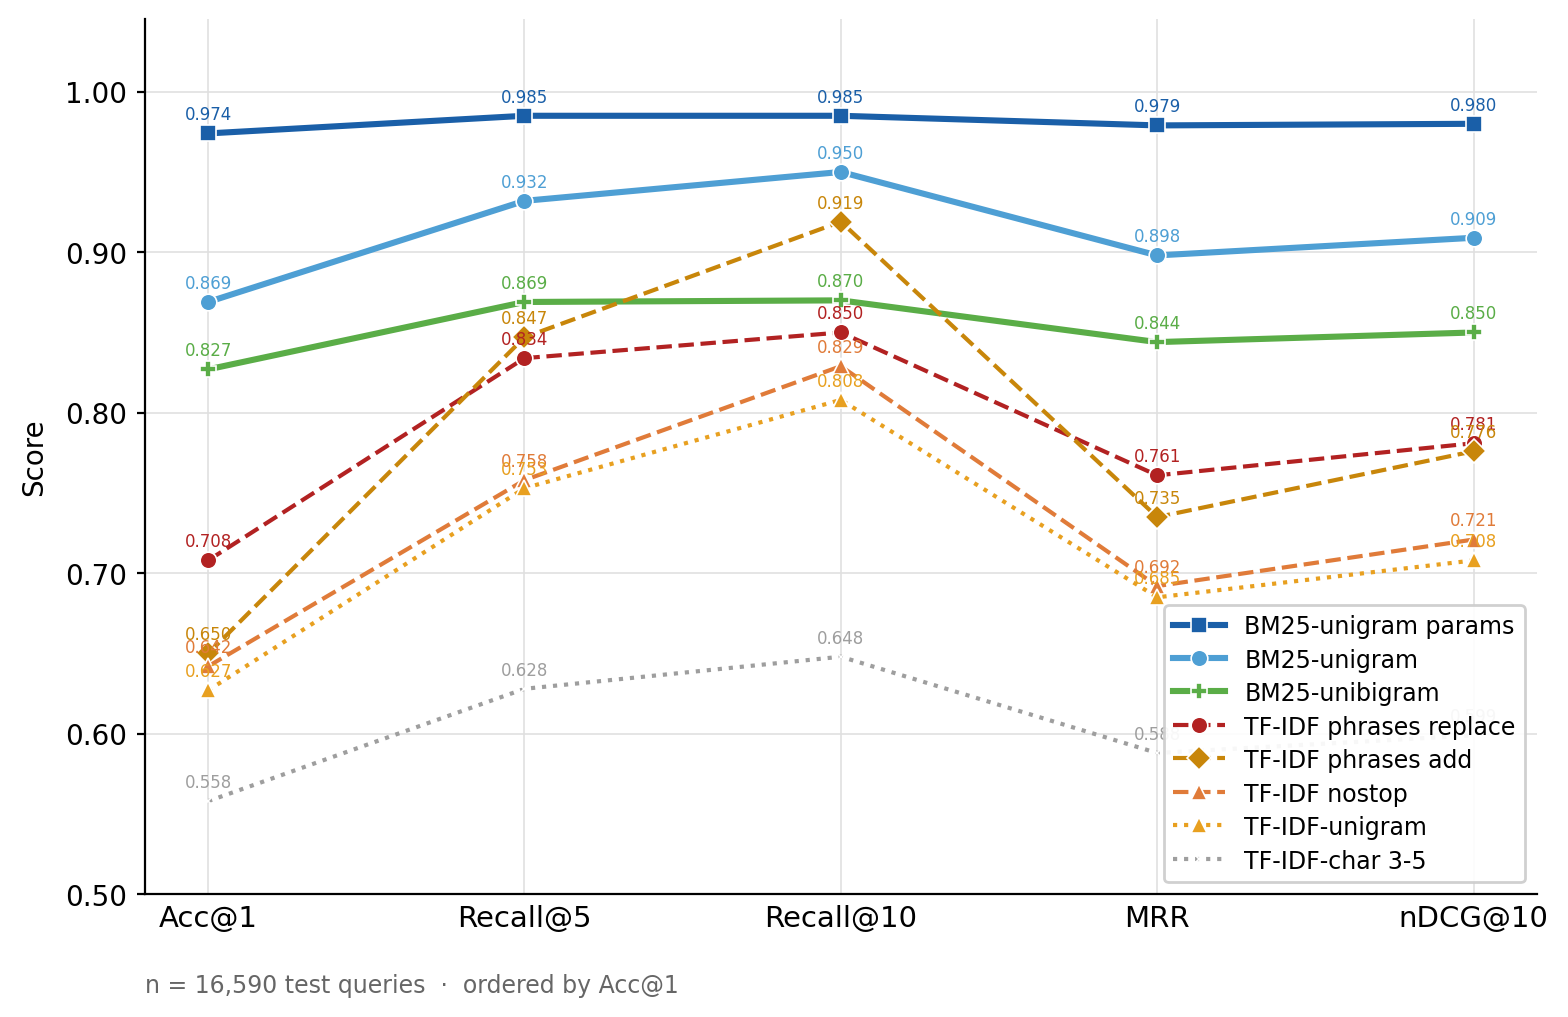
\includegraphics[width=\textwidth]{lexical_performance_item.png}
\caption{Performance comparison of lexical retrieval methods at item level on the test set (n=16,590 queries). Methods are ranked by Accuracy@1.}
\label{fig:lexical_performance_item}
\end{figure}


Figure~\ref{fig:bm25_heatmap_panel} visualizes the sensitivity of item-level Acc@1 to the BM25 hyperparameters $(k_1, b)$ across the three tokenization variants. The parameter-phrase variant dominates the entire explored grid, not only at its optimum, indicating that domain-aware phrase tokenization provides a structural advantage that is robust to hyperparameter choice. All three variants converge on a preference for low $b$ ($\approx 0.35$), suggesting that aggressive length normalization is counterproductive in this catalog where short and long fields differ systematically rather than randomly.

\begin{figure}[htbp]
\centering
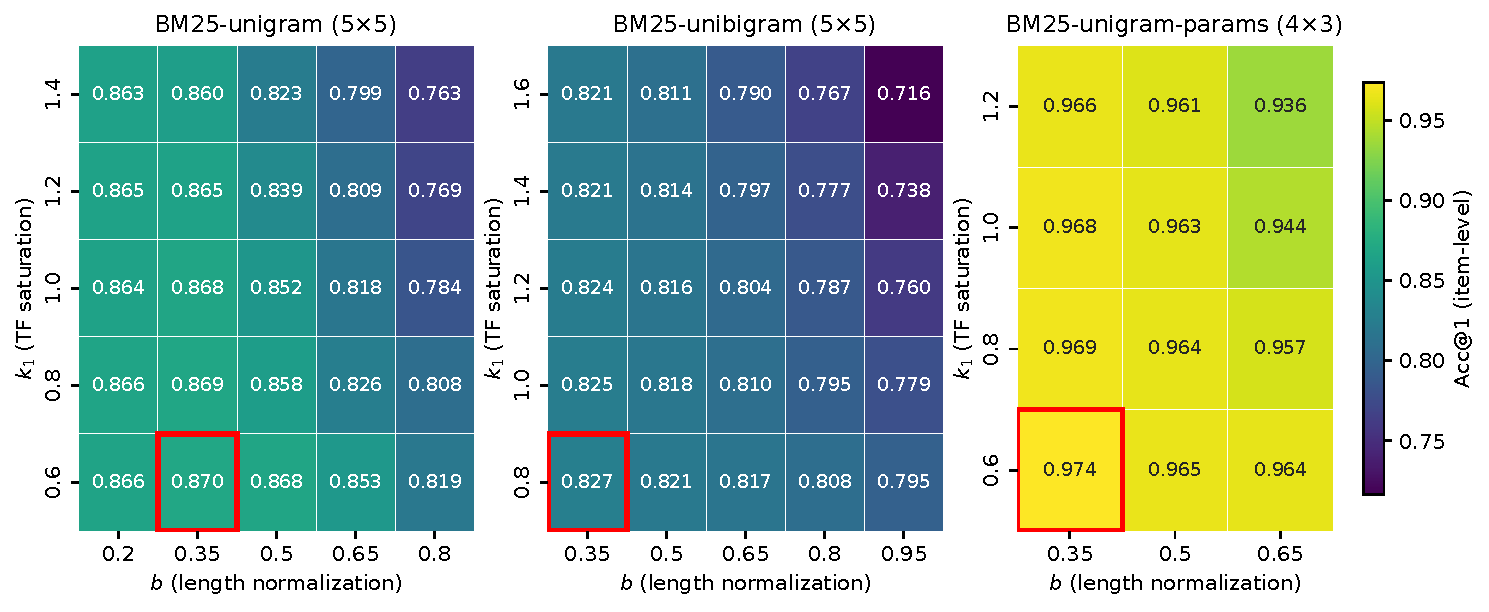
\includegraphics[width=\textwidth]{bm25_heatmap_panel.pdf}
\caption{Acc@1 sensitivity to BM25 hyperparameters ($k_1$, $b$) across three tokenization variants on the item-level retrieval task ($n=16{,}590$ queries). A shared color scale highlights the systematic dominance of the parameter-phrase variant (right panel) across the explored grid. The optimum of each panel is highlighted with a red border.}
\label{fig:bm25_heatmap_panel}
\end{figure}

Bootstrap significance testing (10,000 iterations, Bonferroni correction) confirmed all pairwise differences were statistically significant ($p < 0.003$).  

Table~\ref{tab:statistical_significance} presents pairwise comparisons. BM25-unigram outperformed all TF-IDF variants by 16.1--31.1 percentage points, and exceeded BM25-unibigram by 4.2 percentage points.

\begin{table}[htbp]
\centering
\caption{Pairwise statistical significance testing results for item-level lexical method performance. Bootstrap test with 10,000 iterations; p-values corrected using Holm-Bonferroni method. All comparisons show significant differences ($p < 0.003$).}
\label{tab:statistical_significance}
\resizebox{\textwidth}{!}{%
\begin{tabular}{llrrrr}
\toprule
Method 1 & Method 2 & $\Delta$ Acc@1 & 95\% CI & p-value & Sig. \\
\midrule
BM25-unigram & BM25-unibigram & 0.042 & [0.036, 0.048] & $< 0.001$ & *** \\
BM25-unigram & TF-IDF-phrases\_replace & 0.161 & [0.153, 0.169] & $< 0.001$ & *** \\
BM25-unigram & TF-IDF-phrases\_add & 0.219 & [0.211, 0.227] & $< 0.001$ & *** \\
BM25-unigram & TF-IDF-nostop & 0.227 & [0.220, 0.235] & $< 0.001$ & *** \\
BM25-unigram & TF-IDF-unigram & 0.243 & [0.235, 0.250] & $< 0.001$ & *** \\
BM25-unigram & TF-IDF-char\_3\_5 & 0.311 & [0.303, 0.319] & $< 0.001$ & *** \\
\midrule
BM25-unibigram & TF-IDF-phrases\_replace & 0.118 & [0.112, 0.125] & $< 0.001$ & *** \\
BM25-unibigram & TF-IDF-phrases\_add & 0.177 & [0.170, 0.184] & $< 0.001$ & *** \\
BM25-unibigram & TF-IDF-nostop & 0.185 & [0.178, 0.192] & $< 0.001$ & *** \\
BM25-unibigram & TF-IDF-unigram & 0.200 & [0.193, 0.207] & $< 0.001$ & *** \\
BM25-unibigram & TF-IDF-char\_3\_5 & 0.268 & [0.261, 0.276] & $< 0.001$ & *** \\
\midrule
TF-IDF-phrases\_replace & TF-IDF-phrases\_add & 0.058 & [0.053, 0.064] & $< 0.001$ & *** \\
TF-IDF-phrases\_replace & TF-IDF-nostop & 0.067 & [0.061, 0.072] & $< 0.001$ & *** \\
TF-IDF-phrases\_replace & TF-IDF-unigram & 0.082 & [0.076, 0.088] & $< 0.001$ & *** \\
TF-IDF-phrases\_replace & TF-IDF-char\_3\_5 & 0.150 & [0.143, 0.157] & $< 0.001$ & *** \\
\midrule
TF-IDF-nostop & TF-IDF-phrases\_add & 0.008 & [0.003, 0.014] & $< 0.003$ & ** \\
TF-IDF-unigram & TF-IDF-nostop & 0.015 & [0.010, 0.020] & $< 0.001$ & *** \\
TF-IDF-unigram & TF-IDF-phrases\_add & 0.023 & [0.019, 0.027] & $< 0.001$ & *** \\
\bottomrule
\multicolumn{6}{l}{\small *** $p < 0.001$; ** $p < 0.01$ (Holm-Bonferroni corrected)}
\end{tabular}
}
\end{table}

Stratification by query type (Table~\ref{tab:performance_by_numbers}) revealed that BM25-params achieved perfect accuracy on non-numeric queries (0.17\% of test set) while maintaining 0.974 on numeric ones. TF-IDF variants showed the inverse: perfect non-numeric but weaker numeric performance (0.558--0.708).

\begin{table}[htbp]
\centering
\caption{Item-level performance stratification by query type. The test set comprises 16,076 queries with numbers (99.83\%) and 29 queries without numbers (0.17\%).}
\label{tab:performance_by_numbers}
\resizebox{\textwidth}{!}{%
\begin{tabular}{lrrrr}
\toprule
 & \multicolumn{2}{c}{Acc@1} & \multicolumn{2}{c}{Recall@10} \\
\cmidrule(lr){2-3} \cmidrule(lr){4-5}
Method & Numeric & Non-numeric & Numeric & Non-numeric \\
\midrule
BM25-unigram\_params (k1=0.60, b=0.35) & 0.974 & 1.000 & 0.985 & 1.000 \\
BM25-unigram (k1=0.80, b=0.35) & 0.869 & 0.931 & 0.950 & 1.000 \\
BM25-unibigram (k1=0.80, b=0.35) & 0.826 & 0.966 & 0.870 & 0.966 \\
TF-IDF-unigram\_phrases\_replace & 0.708 & 1.000 & 0.850 & 1.000 \\
TF-IDF-unigram\_phrases\_add & 0.649 & 1.000 & 0.919 & 1.000 \\
TF-IDF-unigram\_nostop & 0.641 & 1.000 & 0.829 & 1.000 \\
TF-IDF-unigram & 0.626 & 1.000 & 0.807 & 1.000 \\
TF-IDF-char\_3\_5 & 0.558 & 1.000 & 0.647 & 1.000 \\
\bottomrule
\end{tabular}
}
\end{table}

Based on item-level results, BM25 with optimized parameters (k1=0.60, b=0.35) was selected as the best-performing lexical method for subsequent pseudo-relevance feedback experiments, demonstrating superior item-level performance across all evaluation metrics with statistical significance.

\FloatBarrier
\subsection{Pseudo-Relevance Feedback Methods}

Pseudo-relevance feedback (PRF) methods were evaluated to assess their effectiveness in enhancing retrieval performance beyond the base lexical retriever. Two PRF approaches were tested: RM3 (Relevance Model 3) and Rocchio feedback. Both methods leveraged BM25-unigram (k1=0.80, b=0.35) as their base retriever, which achieved Acc@1 of 0.869, Recall@5 of 0.932, Recall@10 of 0.950, MRR of 0.898, and nDCG@10 of 0.909 at the item level.

\subsubsection{RM3 and Rocchio Performance}

Six configurations each were evaluated for RM3 and Rocchio, varying feedback documents ($M \in \{5, 10\}$), expansion terms ($N \in \{20, 40\}$), and interpolation weights. Tables~\ref{tab:rm3_configurations} and~\ref{tab:rocchio_configurations} present detailed results. RM3 showed remarkable stability across configurations (Acc@1: 0.8693--0.8699), while Rocchio performance degraded notably with N=40 terms (Acc@1 dropping from 0.857 to 0.837).

\begin{table}[htbp]
\centering
\caption{Performance of RM3 configurations at item level on the test set (n=16,590 queries). All configurations use BM25-unigram as the base retriever.}
\label{tab:rm3_configurations}
\begin{tabular}{cccccc}
\toprule
M & N & $\lambda$ & MRR & nDCG@10 & Acc@1 \\
\midrule
5 & 20 & 0.5 & 0.8983 & 0.9093 & 0.8699 \\
5 & 20 & 0.7 & 0.8982 & 0.9092 & 0.8698 \\
5 & 40 & 0.5 & 0.8982 & 0.9092 & 0.8699 \\
10 & 20 & 0.5 & 0.8983 & 0.9093 & 0.8699 \\
10 & 20 & 0.7 & 0.8978 & 0.9089 & 0.8693 \\
10 & 40 & 0.5 & 0.8982 & 0.9092 & 0.8699 \\
\bottomrule
\end{tabular}
\end{table}

\begin{table}[htbp]
\centering
\caption{Performance of Rocchio configurations at item level on the test set (n=16,590 queries). All configurations use BM25-unigram as the base retriever.}
\label{tab:rocchio_configurations}
\begin{tabular}{cccccc}
\toprule
M & N & $\beta$ & MRR & nDCG@10 & Acc@1 \\
\midrule
5 & 20 & 0.5 & 0.8875 & 0.9000 & 0.8565 \\
5 & 20 & 0.7 & 0.8874 & 0.8999 & 0.8563 \\
5 & 40 & 0.5 & 0.8718 & 0.8877 & 0.8373 \\
10 & 20 & 0.5 & 0.8873 & 0.9000 & 0.8559 \\
10 & 20 & 0.7 & 0.8872 & 0.8999 & 0.8559 \\
10 & 40 & 0.5 & 0.8713 & 0.8873 & 0.8361 \\
\bottomrule
\end{tabular}
\end{table}

\subsubsection{Comparative Analysis and Statistical Significance}

Table~\ref{tab:prf_comparison} presents the performance comparison between the best PRF methods and their base retriever. Statistical significance testing was conducted using paired bootstrap resampling with 10,000 iterations and $\alpha$=0.05, with multiple testing correction using the Holm--Bonferroni method.

\begin{table}[htbp]
\centering
\caption{Comparison of best PRF methods versus base retriever at item level. Statistical significance was assessed using bootstrap resampling (10,000 iterations) with Holm--Bonferroni correction.}
\label{tab:prf_comparison}
\resizebox{\textwidth}{!}{%
\begin{tabular}{lcccc}
\toprule
Method & MRR & nDCG@10 & Acc@1 & Significance \\
\midrule
Base BM25-unigram & 0.898 & 0.909 & 0.869 & --- \\
Best RM3 (M=10, N=20, $\lambda$=0.5) & 0.898 & 0.909 & 0.870 & n.s. \\
Best Rocchio (M=5, N=20, $\beta$=0.5) & 0.888 & 0.900 & 0.857 & $p < 0.05$ \\
\bottomrule
\end{tabular}
}
\end{table}

Table~\ref{tab:prf_comparison} summarizes the comparison. RM3 showed no statistically significant improvement over the baseline (95\% CI: [-0.0005, 0.0021]). Rocchio produced significant degradation ($p < 0.05$, $\Delta=1.26\%$), suggesting that query expansion is ill-suited for this domain where precise numeric matching outweighs semantic expansion.

The strong baseline BM25 performance leaves minimal room for improvement through query expansion, indicating limited value of PRF for this technical retrieval task.

\subsection{Neural Dense Retrieval Methods}

This subsection presents the comparative performance of neural dense retrieval models across three model families: E5, GTE, and BGE-M3. All models were evaluated in zero-shot mode on the same test set of 16,590 queries at both item-level and parent-level retrieval tasks.

\subsubsection{E5 Model Family Performance}

Table~\ref{tab:e5_performance} presents the performance comparison across E5 model variants. The multilingual-e5-base model achieved item-level Acc@1 of 0.134 (13.4\%), meaning only 1 in 7.5 queries successfully retrieved the correct item as the top result. At the parent level, E5-large demonstrated substantially stronger performance with Acc@1 of 0.982 (98.2\%).

\begin{table}[htbp]
\centering
\caption{Performance comparison of E5 model variants. All models evaluated on 16,589 queries (test set).}
\label{tab:e5_performance}
\begin{tabular}{lccccc}
\hline
\textbf{Model} & \textbf{Acc@1} & \textbf{Recall@5} & \textbf{Recall@10} & \textbf{MRR} & \textbf{nDCG@10} \\
\hline
\multicolumn{6}{c}{\textit{Item-Level Retrieval}} \\
\hline
E5-large & 0.134 & 0.376 & 0.518 & 0.251 & 0.303 \\
\hline
\multicolumn{6}{c}{\textit{Parent-Level Retrieval}} \\
\hline
E5-large & 0.982 & 0.993 & 0.996 & 0.987 & 0.969 \\
\hline
\end{tabular}
\end{table}

The E5 model demonstrated dramatically different performance between hierarchical levels, with Acc@1 improving 7.3-fold from 13.4\% at item-level to 98.2\% at parent-level. This pattern suggests that while E5 embeddings effectively capture high-level semantic similarity for parent document matching, they struggle to discriminate between fine-grained item variations within the same parent category.

Stratification by query type revealed a critical limitation: queries without numeric parameters achieved Acc@1 of 0.875 versus 0.133 for numeric queries --- a pattern that persists across all neural model families.

\subsubsection{GTE Model Family Performance}

Table~\ref{tab:gte_performance} presents results for both GTE model variants: the base Alibaba-NLP/gte-multilingual-base model and the instruction-following Alibaba-NLP/gte-multilingual-base instruct variant. Contrary to expectations that the larger instruction-tuned model would demonstrate superior performance, the base GTE-large model outperformed the instruct variant at the parent level while showing marginal improvement at the item level.

\begin{table}[htbp]
\centering
\caption{Performance comparison of GTE model variants with different query formulations.}
\label{tab:gte_performance}
\resizebox{\textwidth}{!}{%
\begin{tabular}{lccccc}
\hline
\textbf{Model} & \textbf{Acc@1} & \textbf{Recall@5} & \textbf{Recall@10} & \textbf{MRR} & \textbf{nDCG@10} \\
\hline
\multicolumn{6}{c}{\textit{Item-Level Retrieval}} \\
\hline
GTE-large-en-v1.5 & 0.013 & 0.044 & 0.066 & 0.030 & 0.036 \\
GTE-Qwen2-instruct & 0.014 & 0.049 & 0.074 & 0.034 & 0.040 \\
\hline
\multicolumn{6}{c}{\textit{Parent-Level Retrieval}} \\
\hline
GTE-large-en-v1.5 & 0.837 & 0.941 & 0.961 & 0.884 & 0.701 \\
GTE-Qwen2-instruct & 0.697 & 0.938 & 0.978 & 0.798 & 0.651 \\
\hline
\end{tabular}
}
\end{table}

Both GTE variants achieved the poorest item-level performance among neural families (Acc@1: 1.3--1.4\%). At the parent level, GTE-large reached 0.837, but the instruction-tuned variant unexpectedly degraded to 0.697, suggesting that explicit prompts introduce noise in structured technical retrieval tasks.

Non-numeric queries showed substantial improvements (GTE-Qwen2: 37.9\% vs 1.4\% overall), reinforcing the numeric precision challenge observed with E5.

\subsubsection{BGE-M3 Multi-Representation Architecture}

Table~\ref{tab:bgem3_performance} presents performance across three retrieval modes of the BGE-M3 unified architecture: dense single-vector, learned sparse representations, and multi-vector ColBERT-style interactions. The multi-vector mode demonstrated substantially superior item-level performance compared to both single-vector approaches.

\begin{table}[htbp]
\centering
\caption{Performance comparison of BGE-M3 retrieval modes. All modes use the same base encoder (568M parameters) with mode-specific output layers.}
\label{tab:bgem3_performance}
\resizebox{\textwidth}{!}{%
\begin{tabular}{lccccc}
\hline
\textbf{Mode} & \textbf{Acc@1} & \textbf{Recall@5} & \textbf{Recall@10} & \textbf{MRR} & \textbf{nDCG@10} \\
\hline
\multicolumn{6}{c}{\textit{Item-Level Retrieval}} \\
\hline
BGE-M3-dense & 0.127 & 0.349 & 0.464 & 0.233 & 0.278 \\
BGE-M3-sparse & 0.125 & 0.401 & 0.535 & 0.252 & 0.309 \\
BGE-M3-colbert & \textbf{0.448} & \textbf{0.753} & \textbf{0.785} & \textbf{0.580} & \textbf{0.630} \\
\hline
\multicolumn{6}{c}{\textit{Parent-Level Retrieval}} \\
\hline
BGE-M3-dense & 0.960 & 0.984 & 0.993 & 0.971 & 0.906 \\
BGE-M3-sparse & \textbf{0.994} & \textbf{0.999} & \textbf{1.000} & \textbf{0.996} & \textbf{0.983} \\
BGE-M3-colbert & 0.997 & 0.999 & 1.000 & 0.998 & 0.958 \\
\hline
\end{tabular}
}
\end{table}

At the item level, BGE-M3-ColBERT achieved Acc@1 of 0.448 (44.8\%), dramatically outperforming the dense mode at 0.127 (12.7\%) and sparse mode at 0.125 (12.5\%). This represents a 3.5-fold improvement over both single-vector approaches. The ColBERT multi-vector approach also substantially outperformed all E5 and GTE variants, achieving 3.3-fold higher Acc@1 than E5-large (0.134) and 34-fold higher Acc@1 than GTE-large (0.013).

Dense and sparse modes converged at nearly identical accuracy (12.5--12.7\%), suggesting that single-vector compression encounters similar limitations regardless of representation strategy.

At the parent level, all three modes demonstrated strong performance exceeding 96\% Acc@1, with the ColBERT mode achieving the highest accuracy at 0.997 (99.7\%), followed closely by sparse at 0.994 (99.4\%) and dense at 0.960 (96.0\%). The narrow ColBERT-over-sparse margin at the parent level (99.7\% vs 99.4\%) suggests that token-level late interaction adds only marginal value when the task reduces to family identification, where learned sparse representations already capture the discriminative lexical patterns necessary for parent-level categorization while maintaining interpretability advantages over dense vectors.

On non-numeric queries, ColBERT and sparse modes achieved perfect accuracy (1.000), while numeric query performance dropped substantially (ColBERT: 44.7\%, sparse/dense: ~12.5\%), confirming ColBERT's relative robustness to numeric constraints.

\subsubsection{Cross-Family Performance Comparisons}

Table~\ref{tab:neural_comparison} presents a direct comparison of item-level Acc@1 performance across the best-performing configuration from each model family, revealing substantial performance differences.

\begin{table}[htbp]
\centering
\caption{Item-level Acc@1 comparison across neural model families. Values shown for best configuration within each family.}
\label{tab:neural_comparison}
\begin{tabular}{lcc}
\hline
\textbf{Model Family} & \textbf{Best Configuration} & \textbf{Acc@1} \\
\hline
BGE-M3 & ColBERT (multi-vector) & 0.448 (44.8\%) \\
E5 & multilingual-e5-large & 0.134 (13.4\%) \\
GTE & gte-large-en-v1.5 & 0.013 (1.3\%) \\
\hline
\multicolumn{3}{l}{\textit{Single-vector modes within BGE-M3:}} \\
BGE-M3 & Sparse & 0.125 (12.5\%) \\
BGE-M3 & Dense & 0.127 (12.7\%) \\
\hline
\end{tabular}
\end{table}

The performance hierarchy is clear: BGE-M3-ColBERT (44.8\%) outperformed E5-large by 31.4 percentage points and GTE-large by 43.5 percentage points. These substantial differences are meaningful for practical retrieval applications.

\subsubsection{Best Neural Models Selected}

BGE-M3-ColBERT emerged as the best neural approach (Acc@1=44.8\%), achieving 3.3-fold and 34-fold improvements over E5-large and GTE-large respectively. However, even this best neural method retrieved the correct item in less than half of queries.

At the parent level, all neural approaches exceeded 96\% Acc@1, confirming that neural models capture broad semantic categories effectively but struggle with fine-grained item-level distinctions.

\subsection{Hybrid Fusion Results}

Table~\ref{tab:hybrid_fusion} presents the performance of the best-performing configurations identified through the parameter sweep for each fusion strategy. All optimal configurations converged on $\beta_{\text{exact}}=0.1$ and $\beta_{\text{overlap}}=0.0$.

\begin{table}[h]
\centering
\caption{Performance of hybrid fusion methods with optimized weights. All configurations use $\beta_{\text{exact}}=0.1$ and $\beta_{\text{overlap}}=0.0$.}
\label{tab:hybrid_fusion}
\small
\resizebox{\textwidth}{!}{%
\begin{tabular}{@{}llcccc@{}}
\toprule
\textbf{Fusion Strategy} & \textbf{Weight Distribution} & \textbf{Acc@1} & \textbf{R@5} & \textbf{R@10} & \textbf{MRR@10} \\
\midrule
\multicolumn{6}{l}{\textit{Three-way fusions (BM25 + BGE-M3 variant + TF-IDF)}} \\
\midrule
BM25 + ColBERT + TF-IDF & 
\begin{tabular}[t]{@{}l@{}}
BM25: 0.879\\
ColBERT: 0.012\\
TF-IDF: 0.110
\end{tabular} & 0.890 & 0.941 & 0.954 & 0.908 \\
\addlinespace
BM25 + Dense + TF-IDF & 
\begin{tabular}[t]{@{}l@{}}
BM25: 0.879\\
Dense: 0.012\\
TF-IDF: 0.110
\end{tabular} & 0.889 & 0.939 & 0.953 & 0.907 \\
\addlinespace
BM25 + Sparse + TF-IDF & 
\begin{tabular}[t]{@{}l@{}}
BM25: 0.879\\
Sparse: 0.012\\
TF-IDF: 0.110
\end{tabular} & 0.882 & 0.940 & 0.953 & 0.903 \\
\midrule
\multicolumn{6}{l}{\textit{Five-way fusion (BM25 + all BGE-M3 variants + TF-IDF)}} \\
\midrule
BM25 + Multi-BGE + TF-IDF & 
\begin{tabular}[t]{@{}l@{}}
BM25: 0.450\\
ColBERT: 0.033\\
Dense: 0.033\\
Sparse: 0.033\\
TF-IDF: 0.450
\end{tabular} & 0.590 & 0.928 & 0.963 & 0.730 \\
\bottomrule
\end{tabular}
}
\end{table}

The three-way fusion configurations yielded Acc@1 scores ranging from $0.882$ to $0.890$, with MRR@10 values between $0.903$ and $0.908$. The BM25 + ColBERT + TF-IDF combination achieved the highest Acc@1 ($0.890$) and MRR@10 ($0.908$). 

The five-way fusion produced an Acc@1 of $0.590$ and MRR@10 of $0.730$, representing substantial decreases of $32.8\%$ and $19.6\%$ respectively compared to the best three-way configuration. However, this strategy achieved the highest Recall@10 ($0.963$), exceeding the three-way fusions by approximately 1 percentage point. The optimal weight distribution for the five-way fusion allocated $45.0\%$ each to BM25 and TF-IDF, with the three BGE-M3 variants receiving equal $3.3\%$ weights.
This weight distribution is itself revealing: the optimizer heavily constrained the neural signals, assigning a collective weight of only $9.9\%$ to all three BGE-M3 variants combined. This distribution suggests that within this highly homogeneous domain, dense neural embeddings offer limited discriminative information beyond what lexical models (BM25 and TF-IDF) capture at the granular item level. Furthermore, given the significant drop in Acc@1, even this minor contribution of neural scores appears sufficient to disrupt top-rank precision. Conversely, the elevated Recall@10 of the five-way fusion confirms that neural signals remain valuable for broader retrieval. This behavior is consistent with the parent-level performance observed across all neural configurations, demonstrating that dense embeddings are effective for coarse-grained localization but struggle with fine-grained item discrimination.


\subsection{Cross-Encoder Reranking}
Cross-encoder reranking was applied to the top-100 candidates from three retrieval systems: BM25 (unigram), the hybrid approach (BM25 + BGE-ColBERT + TF-IDF character n-grams), and BGE-M3-ColBERT. Two reranking strategies were evaluated: \textit{replace}, which uses cross-encoder scores exclusively to rerank candidates, and \textit{blend}, which combines original retrieval scores with cross-encoder scores using weighted interpolation ($\lambda=0.6$)).

Table~\ref{tab:reranking_results} presents the performance of both reranking strategies for each retrieval system.
\begin{table}[ht]
\centering
\caption{Performance comparison of cross-encoder reranking strategies. Replace uses CE scores only; Blend combines original retrieval scores with CE scores ($\lambda=0.6$).}
\label{tab:reranking_results}
\resizebox{\textwidth}{!}{%
\begin{tabular}{lcccc}
\hline
\textbf{System} & \textbf{Acc@1} & \textbf{Recall@5} & \textbf{Recall@10} & \textbf{MRR@10} \\
\hline
\textit{BM25 (unigram)} & & & & \\
\quad Baseline & 0.869 & 0.931 & 0.950 & 1.000 \\
\quad Replace & 0.434 & 0.841 & 0.916 & 0.607 \\
\quad Blend & 0.766 & 0.942 & 0.966 & 0.845 \\
\hline
\textit{BGE-M3-ColBERT} & & & & \\
\quad Baseline & 0.448 & 0.753 & 0.785 & 0.580 \\
\quad Replace & 0.299 & 0.664 & 0.740 & 0.455 \\
\quad Blend & 0.475 & 0.764 & 0.786 & 0.601 \\
\hline
\textit{Hybrid (BM25 + BGE-ColBERT + TF-IDF)} & & & & \\
\quad Baseline & 0.590 & 0.928 & 0.963 & 0.730 \\
\quad Replace & 0.430 & 0.858 & 0.932 & 0.608 \\
\quad Blend & \textbf{0.799} & \textbf{0.985} & \textbf{0.988} & \textbf{0.885} \\
\hline
\end{tabular}
}
\end{table}
The blend strategy consistently outperformed the replace strategy across all three systems. For BM25 (unigram), blend achieved Acc@1 of 0.766 compared to 0.434 for replace, representing an improvement of +0.332. The hybrid system with blend reranking achieved the highest overall performance: 0.799 Acc@1, 0.985 Recall@5, 0.988 Recall@10, and 0.885 MRR@10, with improvements of +0.369, +0.127, +0.056, and +0.277 respectively over replace. BGE-M3-ColBERT blend showed improvements of +0.176 in Acc@1 and +0.146 in MRR@10 compared to replace.

The blend strategy consistently outperformed replace across all systems, demonstrating that combining original retrieval signals with cross-encoder scores is essential.

\subsection{Error Analysis}
\label{subsec:error_analysis}

To understand the failure modes of each retrieval approach, we conducted a detailed error analysis on 100 randomly sampled failures per method. Errors were classified into four categories: \textit{Numeric Mismatch} (different specifications), \textit{Lexical Confusion} (similar terms), \textit{Near-Duplicate Error} (ambiguous entries), and \textit{Other}.

\subsubsection{Error Type Distribution}

Table~\ref{tab:error_distribution} presents the distribution of error types across the three primary retrieval methods. Both BM25 and BGE-M3 ColBERT showed similar profiles, with numeric mismatches accounting for approximately 98\% of failures. The hybrid method showed a distinct profile, with all errors in the ``Other'' category.

\begin{table}[htbp]
\centering
\caption{Error type distribution across retrieval methods (\% of failed queries, $n=100$ per method)}
\label{tab:error_distribution}
\resizebox{\textwidth}{!}{%
\begin{tabular}{lccc}
\toprule
\textbf{Error Type} & \textbf{BM25 Unigram} & \textbf{BGE-M3 ColBERT} & \textbf{Hybrid} \\
\midrule
Numeric Mismatch    & 98.1\%  & 97.9\%  & ---     \\
Lexical Confusion   & 0.5\%   & 0.5\%   & ---     \\
Other               & 1.3\%   & 1.6\%   & 100.0\% \\
\bottomrule
\end{tabular}
}
\end{table}

Figure~\ref{fig:error_distribution} visualizes the same distribution and makes the asymmetry between methods immediately apparent: BM25 and BGE-M3-ColBERT share a near-identical failure profile dominated by numeric mismatches, whereas the hybrid method's failures concentrate entirely in the ``Other'' category. The hybrid fusion thus appears to resolve the numeric- and lexical-confusion failure modes that affect each component method in isolation, but at the cost of introducing a new failure mode analyzed in the following subsections.

\begin{figure}[ht]
\centering
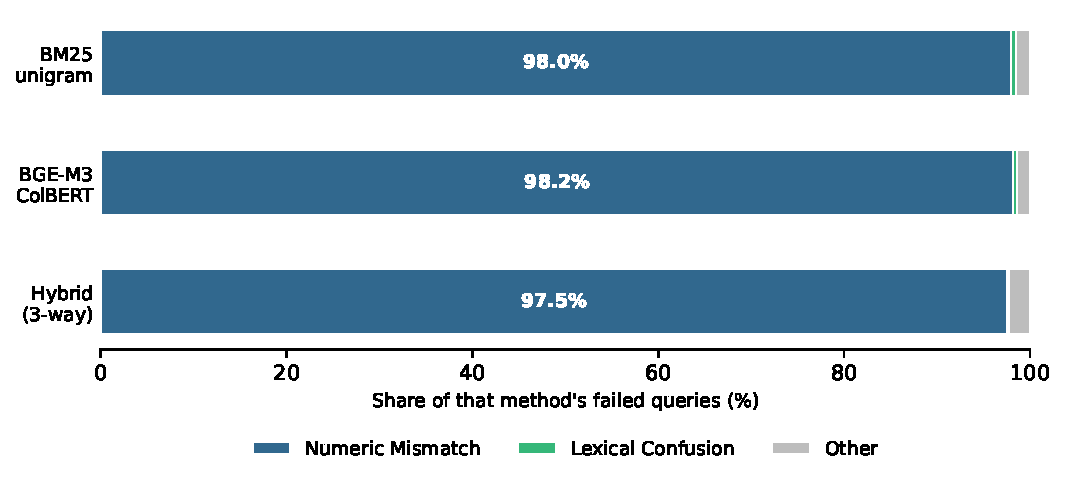
\includegraphics[width=\textwidth]{error_distribution.pdf}
\caption{Error type distribution across the three representative retrieval methods ($n=100$ sampled errors per method). Numeric mismatches dominate both lexical (BM25) and neural (BGE-M3-ColBERT) failures ($\sim 98\%$), revealing a shared blind spot. The hybrid method's failures concentrate entirely in the ``Other'' category, a qualitatively different failure mode discussed in Sec.~\ref{subsec:error_analysis}.}
\label{fig:error_distribution}
\end{figure}

\subsubsection{Hierarchical Error Classification}

Beyond categorical error types, we analyzed failures according to the hierarchical structure of our construction database, where items are organized under parent categories (e.g., OEB280\$ for 40mm polyethylene conduits). Table~\ref{tab:hierarchical_errors} shows three distinct failure patterns: (1) retrieving the correct parent category but wrong specific item variant, (2) retrieving an incorrect parent category entirely, and (3) failing to include the correct parent in the top-10 results.

\begin{table}[htbp]
\centering
\caption{Hierarchical error patterns across retrieval methods}
\label{tab:hierarchical_errors}
\begin{tabular}{lccc}
\toprule
\textbf{Error Pattern} & \textbf{BM25} & \textbf{BGE-M3} & \textbf{Hybrid} \\
 & \textbf{Unigram} & \textbf{ColBERT} & \\
\midrule
Right parent, wrong item & 10.4\%  & 54.3\%  & 36.0\% \\
Wrong parent             & 2.6\%   & 0.3\%   & 3.0\%  \\
Parent not in top-10     & 0.1\%   & 0.0\%   & 0.0\%  \\
\bottomrule
\end{tabular}
\end{table}

The neural method (BGE-M3 ColBERT) demonstrated strong performance at the parent category level, with 54.3\% of errors involving correct parent identification but incorrect item selection --- more than 5× higher than BM25 (10.4\%). This suggests that dense embeddings effectively capture high-level semantic categories but struggle with fine-grained distinctions within categories. Conversely, BM25 exhibited higher wrong-parent rates (2.6\% vs. 0.3\%), indicating occasional failures at the coarse-grained category level. The hybrid approach showed intermediate behavior with 36.0\% right-parent-wrong-item errors.

\subsubsection{Representative Error Examples}

Table~\ref{tab:error_examples} presents representative examples. Numeric mismatches occurred when systems retrieved variants with different specifications (e.g., ``3 tubos'' vs ``5 tubos'') despite matching other attributes. Lexical confusion involved semantically related but distinct terms. ``Other'' errors primarily involved mismatched action verbs or scope modifiers.

\begin{table*}[htbp]
\centering
\caption{Representative error examples by category}
\label{tab:error_examples}
\resizebox{\textwidth}{!}{%
\begin{tabular}{p{0.15\textwidth}p{0.38\textwidth}p{0.38\textwidth}p{0.08\textwidth}}
\toprule
\textbf{Category} & \textbf{Query} & \textbf{Retrieved (Incorrect)} & \textbf{Method} \\
\midrule
\multicolumn{4}{l}{\textit{Numeric Mismatch}} \\
\midrule
OEB290cbebb & Concrete-encased \textbf{3 pipes} polyethylene 50mm under tracks, any shift, $3 \leq i<5$h, low volume & Concrete-encased \textbf{5 pipes} polyethylene 50mm under tracks, any shift, $3 \leq i<5$h, low volume & BM25 \\
\addlinespace
OEB280egecb & Concrete-encased \textbf{5 pipes} polyethylene 40mm in ballast, any shift, \textbf{$i<3$h}, low volume & Concrete-encased \textbf{5 pipes} polyethylene 40mm in ballast, any shift, \textbf{$3 \leq i<5$h}, low volume & BGE-M3 \\
\midrule
\multicolumn{4}{l}{\textit{Lexical Confusion}} \\
\midrule
OEB250abaec & Supply conduit 4 pipes galv.\ steel 100mm CMS transitions, \textbf{exceptional daytime}, N/A, any condition & Supply conduit 4 pipes galv.\ steel 100mm CMS transitions, \textbf{shift: N/A}, maintenance: N/A, any condition & BM25 \\
\addlinespace
OEB120aedc & Conduit entry 1--2 pipes in chamber, \textbf{any shift}, no interval needed, any condition & Conduit entry 1--2 pipes in chamber, \textbf{any exceptional shift}, no interval needed, any condition & BGE-M3 \\
\midrule
\multicolumn{4}{l}{\textit{Other}} \\
\midrule
OEB250bbbcc & \textbf{Supply and installation} conduit 4 pipes steel 100mm CMS, exceptional night, i<3h, any condition & \textbf{Supply} conduit 4 pipes steel 100mm CMS, exceptional night, i<3h, any condition & BM25 \\
\addlinespace
OEB110bda & PVC pipe 110mm chamber drainage, \textbf{night shift}, no interval needed, high volume & PVC pipe 110mm chamber drainage, \textbf{exceptional night}, no interval needed, high volume & BGE-M3 \\
\bottomrule
\end{tabular}
}
\end{table*}

\subsubsection{Method-Specific Error Patterns}

Analysis of near-duplicate handling revealed stark differences between methods. BM25 produced 3,276 duplicate documents across 1,602 duplicate groups in its embedding space, while BGE-M3 ColBERT produced zero duplicates. This difference stems from BM25's purely lexical matching, which assigns identical sparse vectors to textual variants with negligible term frequency differences. The hybrid method, incorporating character n-gram features, eliminated these duplicates while attempting to preserve BM25's numeric discrimination capabilities.

For the hybrid method, the absence of traditional numeric mismatch or lexical confusion errors suggests that its failures occurred at a different stage of processing. The 36\% right-parent-wrong-item rate indicates that while the method successfully identified relevant categories, the fusion mechanism between lexical and semantic signals did not optimally resolve fine-grained distinctions within those categories.

\subsection{Overall Performance Summary}
\label{sec:4.7_Overall Performance Summary}

Figure~\ref{fig:acc1_by_family} consolidates the central finding visually: the best configuration of each method family is plotted at both evaluation levels. Lexical retrieval (BM25-unigram-params) leads at item level by a wide margin, while neural retrieval (BGE-M3-ColBERT) collapses on the same task --- yet recovers to near-perfect performance at parent level. The dramatic item-to-parent gap exhibited by the neural family is the visual signature of the paper's main result: dense embeddings localize the parametric family well but cannot disambiguate variants within it. Parent-level metrics were not computed for the Hybrid and Reranking families in this work and appear as ``n/a''.

\begin{figure}[ht]
\centering
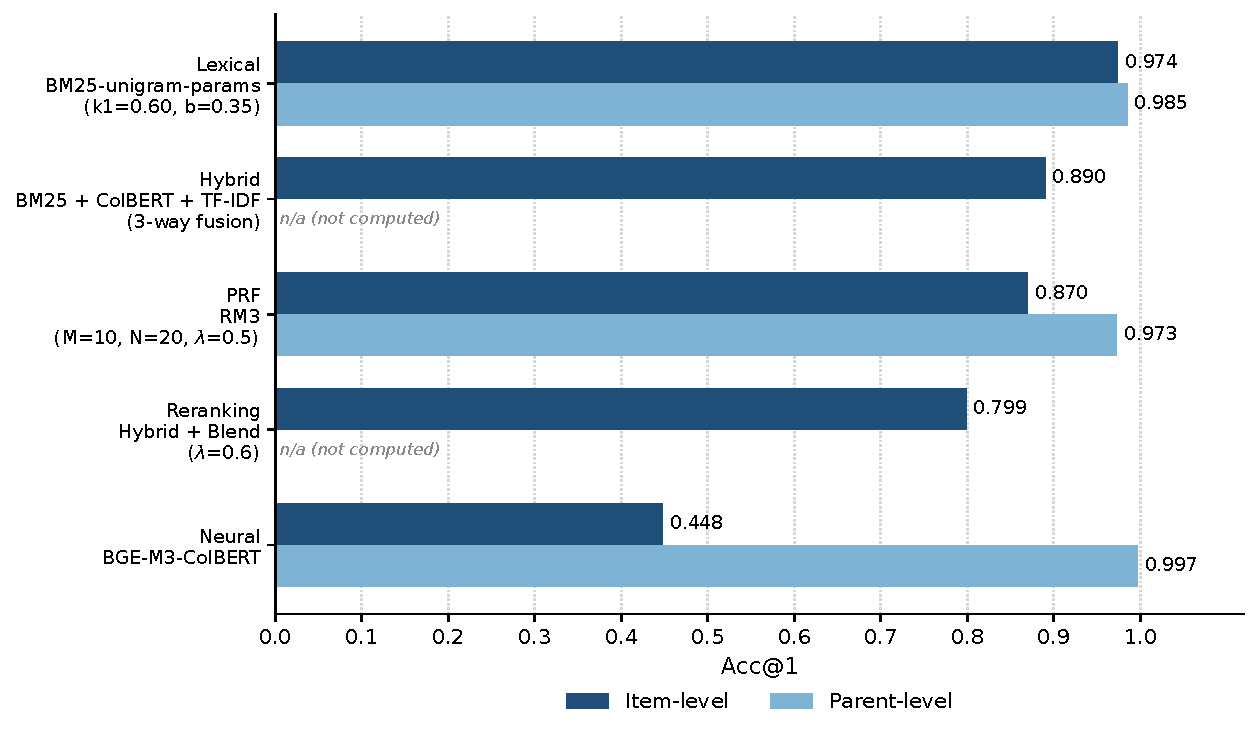
\includegraphics[width=\textwidth]{acc1_by_family.pdf}
\caption{Best Acc@1 per method family at item-level and parent-level on the test set ($n=16{,}590$ queries). For each family, the configuration with the highest item-level Acc@1 was selected and both its item- and parent-level scores are plotted. The 52.6-percentage-point item-level gap between Lexical and Neural collapses at parent-level, where Neural reaches $0.997$. Parent-level results were not computed for the Hybrid and Reranking families in this work (marked ``n/a''); a full parent-level evaluation of these families is deferred to future work.}
\label{fig:acc1_by_family}
\end{figure}

Table~\ref{tab:overall_performance} presents the top-performing configurations across all evaluated retrieval methods, ranked by Acc@1. The table encompasses lexical methods, pseudo-relevance feedback approaches, neural retrievers, hybrid fusion strategies, and reranked systems.

\begin{table}[htbp]
\centering
\caption{Top 10 retrieval configurations ranked by Acc@1 on the test set (n=16,590 queries). MRR values provided for reference.}
\label{tab:overall_performance}
\begin{tabular}{lcc}
\toprule
\textbf{Configuration} & \textbf{Acc@1} & \textbf{MRR} \\
\midrule
BM25-unigram\_params (k1=0.60, b=0.35) & 0.974 & 0.979 \\
BM25 + ColBERT + TF-IDF (3-way fusion) & 0.890 & 0.908 \\
BM25 + Dense + TF-IDF (3-way fusion) & 0.889 & 0.907 \\
BM25 + Sparse + TF-IDF (3-way fusion) & 0.882 & 0.903 \\
RM3 (M=5, N=20, $\lambda$=0.5) & 0.870 & 0.898 \\
BM25-unigram (default, k1=0.80, b=0.35) & 0.869 & 0.898 \\
Rocchio (M=5, N=20, $\beta$=0.5) & 0.857 & 0.888 \\
BM25-unibigram (k1=0.80, b=0.35) & 0.827 & 0.844 \\
5-way fusion + Blend reranking & 0.799 & 0.885 \\
BM25 + Blend reranking & 0.766 & 0.845 \\
\midrule
\multicolumn{3}{l}{\textit{Best neural (for reference):}} \\
BGE-M3-ColBERT & 0.448 & 0.580 \\
\bottomrule
\end{tabular}
\end{table}

The evaluation across 100 configurations produced four findings: (1) optimized BM25 achieved the highest performance (Acc@1=97.4\%); (2) the best neural approach underperformed by 52.6 percentage points; (3) hybrid fusion nearly doubled neural-only performance ($89.0\%$ vs $44.8\%$); and (4) cross-encoder reranking improved results but did not surpass the lexical baseline.
These rankings are based on Acc@1, which reflects automated deployment scenarios where only the top result is used. Practitioners operating in semi-automated workflows — where a human reviewer examines the first few candidates — may find Recall@5 or MRR more relevant criteria and, under those metrics, hybrid configurations show comparatively stronger performance relative to the lexical baseline, as reflected in Table~\ref{tab:overall_performance}.


\section{Discussion}
\label{sec:discussion}

Our results reaffirm the strength of lexical methods in specialized technical domains. A well-tuned BM25 configuration significantly outperformed all neural retrievers at the item level, achieving approximately 97.4\% Acc@1 on a 40,000-item catalog. This aligns with prior findings that optimized lexical models often surpass neural approaches in domain-specific settings with consistent terminology ~\cite{thakur2021beir}, and echoes work showing that term dictionaries improve AEC search precision ~\cite{fan2015project}. For practitioners, the implications are clear: BM25 offers high accuracy with minimal infrastructure and sub-second latency, making it a cost-effective and scalable solution for catalog retrieval.

Neural retrievers, by contrast, excel at high-level semantic categorization but struggle with fine-grained item matching. At the parent level, models like BGE-M3-ColBERT achieved approximately 99.7\% accuracy, rivaling lexical methods; however, at the item level, their performance lagged due to vocabulary mismatch and lack of domain adaptation. General-purpose embeddings underperform on specialized tasks because they handle rare terms poorly ~\cite{tang2024we}, and dense retrievers generalize poorly without fine-tuning ~\cite{li2022domain}. Construction catalogs combine technical jargon, codes, and measurements infrequent in general corpora—terms BM25 handles well via inverse document frequency. It is worth noting that this comparison is intentionally asymmetric in one respect: while BM25 was tuned with domain-specific parameter phrases and optimized hyperparameters, neural models were evaluated in zero-shot mode without any domain adaptation. This reflects a realistic deployment scenario where labeled training data is unavailable, and where lexical methods can be configured with modest domain knowledge at low cost. Even if domain adaptation were to narrow this gap, practitioners would still need to weigh the added complexity and computational cost of neural retrievers against the simplicity and transparency of a well-tuned BM25 system.

Hybrid methods improved performance but did not outperform standalone BM25, diverging from general-domain findings where convex combination fusion often outperforms reciprocal rank fusion with minimal training data ~\cite{bruch2023analysis}. In our setting, BM25's near-optimal accuracy left little headroom for neural signals to contribute meaningfully, suggesting that hybridization may introduce noise in highly technical domains. Learned sparse methods like SPLADE offer a compromise by combining semantic understanding with sparse term expansions ~\cite{formal2021splade}; our BGE-sparse variant rivaled ColBERT at parent level, though SPLADE's complexity remains a deployment barrier.

Cross-encoder reranking showed mixed results. The replace strategy degraded BM25 from $0.869$ to $0.434$ Acc@1, suggesting that general-domain reranking models struggle to distinguish fine-grained technical differences in parametric catalog entries. The blend strategy ($\lambda=0.6$) proved more effective, with a hybrid system achieving 0.799 Acc@1. However, BM25 with blend (0.766) still underperformed standalone BM25, suggesting reranking offers limited value when lexical baselines are already strong ~\cite{nogueiraDocumentRankingPretrained2020, zhuang2023rankt5}.

Error analysis revealed systematic patterns. Neural retrievers struggled with numeric precision: BERT's subword tokenization breaks numbers into fragments, impairing magnitude representation ~\cite{wallace2019nlp}—explaining why approximately 98\% of neural errors involved numeric mismatches. Many catalog items are near-duplicates differing only in minor attributes, and single-vector models struggled with these fine distinctions whereas ColBERT performed better yet still trailed lexical methods on exact matches. Construction documents combine structured codes with technical free text, and NLP tools tailored to construction yield high precision by leveraging both cues ~\cite{AKANBI2021}, while specifications encode procedural logic often ignored by generic retrievers ~\cite{LI2023}. BM25 benefits from transparent matching but remains brittle to synonyms; neural models bridge this gap but introduce opacity.

Prior work focused on classification using rule-based and ML approaches ~\cite{caldasAutomatingHierarchicalDocument2003, natural_wu_2022, martinez-rojasApproachAutomaticClassification2015, role_martnezrojas_2016, martinez-rojasUsingClassificationTechniques2018}, but these studies use small datasets and do not benchmark retrieval across method families. Recent work has noted persistent challenges with construction-specific jargon ~\cite{natural_wu_2022} and domain adaptation for language models ~\cite{chungComparingNaturalLanguage2023}. Our study fills this gap by systematically evaluating retrieval on a large-scale catalog, where fine-grained matching reveals effectiveness differences invisible at the category level.

For industry applications, domain-tuned lexical retrieval should be the default. We recommend implementing optimized BM25 with domain-aware preprocessing, conducting targeted error analysis, and exploring neural reranking only when limitations stem from semantic gaps rather than terminology mismatches. Improving data quality often delivers greater returns than model complexity; if neural approaches are pursued, pseudo-label fine-tuning offers a practical path ~\cite{li2022domain}.

Information retrieval benchmarks must also account for latency and hardware constraints ~\cite{santhanam-etal-2023-moving}. BM25 offers sub-100ms latency on standard hardware, while neural retrievers require GPUs with 2–10× overhead. Lexical methods accommodate catalog updates without retraining, and interpretability favors BM25's transparent term matching over opaque neural scores --- though learned sparse retrievers offer a middle ground ~\cite{bruch2023analysis}. Retrieval capabilities should  be integrated in tools like BIM software to support semi-automated 5D workflows.

This study has several limitations that should be considered when interpreting the results. The dataset used in the experiments covers a single subcategory of the ADIF catalog -specifically, the section dedicated to platform conduit systems (designated as chapter 'OEB')—which, while containing nearly 40,000 parametric variants represents a homogeneous domain where all items follow the same structural template and use the same set of descriptive attributes. This homogeneity may favor lexical methods, as BM25 benefits from consistent terminology and predictable parametric vocabulary. At the same time, the near-identical nature of catalog entries positions this homogeneous catalog as a rigorous benchmark for hard-negative retrieval. Validation across other ADIF catalog chapters — such as track infrastructure or electrification systems, which exhibit greater lexical diversity — would strengthen the generalizability of these findings and is a priority for future work.
Additional limitations include the zero-shot evaluation of neural models. While this setup reflects realistic deployment constraints where annotated domain-specific data is unavailable, it leaves open the question of how much domain-adapted fine-tuning could narrow the performance gap with lexical methods. Furthermore, the cross-encoder employed (ms-marco-MiniLM-L-6-v2) was trained exclusively on English web-search data, and its underperformance may reflect the challenges of cross-lingual domain mismatch, rather than an inherent limitation of the reranking paradigm. The poor performance of GTE model (approximately $1\%$ Acc@1) further illustrates that retrieval in technical domains remains an open challenge ~\cite{jungyeon2024cross-lingual}. Finally, SPLADE was excluded due to limited Spanish language support, and the single-correct-item assumption may oversimplify practical deployment scenarios where multiple catalog entries represent acceptable substitutes.



\section{Conclusions and Future Work}

We presented a systematic evaluation of retrieval methods for construction parametric catalogs, where small lexical or numeric differences determine success. Across 100 configurations and nearly 40,000 real-world Spanish railway catalog items, the central finding is clear: a well-tuned BM25 configuration incorporating domain-specific parameter phrases achieves $97.4\%$ top-1 accuracy, outperforming the best neural retriever (BGE-M3-ColBERT, $44.8\%$) by over 52 percentage points and all hybrid configurations by more than 8 points. Neural models, while competitive at the broad category level, consistently fail on fine-grained parametric variants — with nearly all failures occurring on items that differ from the correct answer only in a numeric technical parameter. These results establish lexical retrieval as the best baseline for this class of precision-critical technical search tasks, and demonstrate that neural methods cannot be assumed to generalize effectively to specialized parametric domains without domain adaptation.


For practitioners deploying search over construction catalogs, we recommend starting from a strong lexical baseline with domain-aware tokenization, synonym maps, and unit normalization—favoring simple, well-instrumented baselines before adopting heavier models. Where precision is critical, a compact cross-encoder on top-$k$ candidates improves Acc@1 with modest cost. Exploiting catalog structure by indexing names, types, brands, and standardized attributes separately proves beneficial, as does operationalizing for change: monitoring drift as catalogs evolve, tracking numeric mismatches and near-duplicates, and preferring swappable components.

Several research directions warrant further investigation. Cross-domain validation across other ADIF catalog chapters and external taxonomies would strengthen generalizability ~\cite{royanoAnalysisClassificationSystems2023a}, while multilingual expansion could address terminology drift and locale-specific conventions ~\cite{valentini2024messirve,tang2024we,jungyeon2024cross-lingual}. Deployment studies examining informal price-driven queries, efficiency–effectiveness trade-offs ~\cite{bruch2023analysis}, and integration with BIM and estimation tools remain necessary, and field validation with construction professionals is essential to assess whether ranking improvements yield measurable productivity gains.

Technical gaps also persist. Neural encoders need specialized tokenization for numbers, tolerances, and unit conversions. Structured vocabularies and ontologies remain underused despite their utility for disambiguation ~\cite{yan2022overview,schlachter2021linked}. Catalog-scale search should optimize both quality and cost/latency ~\cite{bruch2023analysis}, and adversarial probes can expose brittleness and prevent silent failures in safety-critical selections ~\cite{wallace2019nlp}.

Finally, well-measured retrieval is foundational for automation in estimating, compliance checking, and procurement. Our benchmark can accelerate reproducible research, while deployment guidance aims to reduce costly mismatches. However, indiscriminate automation may amplify biases or degrade oversight; we recommend phased rollouts with human-in-the-loop review for high-stakes selections.

\appendix
\section{Supplementary Material}
\label{app:supplementary}

Research data associated with this article will be made available at the following repository:

\begin{itemize}
  \item https://doi.org/10.5281/zenodo.20277801
  \item https://doi.org/10.5281/zenodo.20277824
\end{itemize}

The repository includes:
\begin{itemize}
  \item The full parametric construction catalog dataset used in the experiments
  \item Query sets, evaluation labels, and retrieval outputs
  \item Scripts and configuration files for reproducing the benchmarking results
\end{itemize}

\section{Technical Background on Retrieval Methods}
\label{app:technical-background}

\subsection{Information Retrieval Methods}

\subsubsection{Lexical Methods}

Traditional information retrieval relies on lexical matching between queries and documents through term-based scoring functions. TF-IDF (Term Frequency-Inverse Document Frequency) weighs terms by their frequency within documents and rarity across the collection ~\cite{salton1988term, manning2008introduction}.

BM25 extends TF-IDF with sophisticated length normalization and term frequency saturation ~\cite{robertson2009probabilistic}:
\begin{equation}
\text{BM25}(q,d) = \sum_{t \in q} \text{IDF}(t) \cdot \frac{f(t,d) \cdot (k_1 + 1)}{f(t,d) + k_1 \cdot (1 - b + b \cdot \frac{|d|}{\text{avgdl}})}
\end{equation}
where $f(t,d)$ is the frequency of term $t$ in document $d$, $|d|$ is the document length, $\text{avgdl}$ is the average document length in the collection, $k_1$ controls term frequency saturation (typically 0.9--2.0), and $b$ controls length normalization (typically 0.4--0.8). Recent studies demonstrate that properly tuned BM25 can outperform neural models in specialized domains, particularly when queries and documents share consistent terminology ~\cite{thakur2021beir}. The importance of parameter tuning for BM25 cannot be overstated --- performance can vary significantly across different $k_1$ and $b$ values depending on collection characteristics ~\cite{trotmanImprovementsBM25Language2014}.

Character n-gram variants of TF-IDF provide robustness to spelling variations and partial matches, particularly valuable in technical domains with abbreviations and compound terms ~\cite{mcnameeCharacterNGramTokenization2004}. These methods generate overlapping character sequences (e.g., 3--5 characters), enabling matching even when exact terms differ slightly.

\subsubsection{Pseudo-Relevance Feedback}

Pseudo-relevance feedback (PRF) methods enhance retrieval by assuming top-ranked documents from an initial search are relevant and using them to reformulate queries ~\cite{rocchio1971relevance}.

Relevance Model 3 (RM3) interpolates the original query with a relevance model estimated from top-ranked documents ~\cite{abdul2004umass}:
\begin{equation}
P(t|q') = \lambda P(t|q) + (1-\lambda) \sum_{d \in R} P(t|d) P(d|q)
\end{equation}
where $q'$ is the expanded query, $t$ is a candidate term, $P(t|q)$ is the term probability in the original query, $P(t|d)$ is the term probability in document $d$, $P(d|q)$ is the document relevance score, $R$ is the set of top-ranked pseudo-relevant documents, and $\lambda$ balances original and expansion terms. RM3 consistently improves retrieval effectiveness but requires careful tuning of the number of feedback documents and terms ~\cite{lv2010empirical}.

Rocchio's method adjusts query vectors based on centroids of relevant and non-relevant documents ~\cite{rocchio1971relevance}:
\begin{equation}
\vec{q'} = \alpha \vec{q} + \beta \frac{1}{|R|} \sum_{d \in R} \vec{d} - \gamma \frac{1}{|N|} \sum_{d \in N} \vec{d}
\end{equation}
where $\vec{q}$ and $\vec{q'}$ are the original and modified query vectors, $\vec{d}$ represents document vectors, $R$ and $N$ are the sets of relevant and non-relevant documents respectively, and $\alpha$, $\beta$, $\gamma$ control the influence of each component. While originally designed for vector space models, Rocchio adapts well to modern retrieval systems ~\cite{cao2008selecting}.

\subsubsection{Neural Retrieval Methods}

Modern neural approaches transform the retrieval problem into dense vector similarity search. Bi-encoder architectures independently encode queries and documents into fixed-dimensional representations, enabling efficient similarity computation through inner products or cosine similarity ~\cite{karpukhin2020dense}.

The advent of transformer-based models revolutionized dense retrieval, with BERT-based encoders capturing richer semantic relationships ~\cite{devlin2019bert}. Models like Sentence-BERT adapt BERT for efficient sentence-level encoding through siamese and triplet networks ~\cite{reimers2019sentence}.

Contemporary dense retrieval models include:
\begin{itemize}
\item \textbf{E5 (EmbEddings from bidirEctional Encoder rEpresentations):} Trained with contrastive learning on large-scale pairs, showing strong zero-shot performance ~\cite{wang2024text}
\item \textbf{GTE (General Text Embeddings):} Optimized for diverse retrieval tasks through multi-stage training ~\cite{li2023towards}
\item \textbf{BGE (BAAI General Embedding):} Combines contrastive and distillation learning for robust representations ~\cite{chen2024bge}
\end{itemize}

Sparse neural methods like SPLADE learn term importance weights while maintaining the interpretability of lexical matching ~\cite{formal2021splade}. These models use transformer architectures to predict term weights, effectively learning context-aware term expansion and reweighting.

Late-interaction models balance effectiveness and efficiency through token-level interactions. ColBERT (Contextualized Late Interaction over BERT) encodes queries and documents into bags of contextualized embeddings, computing relevance through the sum of maximum similarities ~\cite{khattab2020colbert}:
\begin{equation}
\text{Score}(q,d) = \sum_{t_q \in q} \max_{t_d \in d} \text{sim}(E_q(t_q), E_d(t_d))
\end{equation}

Recent multi-representation models, such as BGE-M3, combine dense, sparse, and multi-vector strategies within a single framework, adapting to different retrieval scenarios ~\cite{chen2024bge}. These unified models show particular promise for multilingual and domain-specific applications where different representation strategies may excel for different query types.

\subsection{Hybrid and Reranking Approaches}

\subsubsection{Fusion Methods}

Combining multiple retrieval signals often improves performance by leveraging complementary strengths. Reciprocal Rank Fusion (RRF) merges rankings without requiring score calibration ~\cite{cormack2009reciprocal}:
\begin{equation}
\text{RRF}(d) = \sum_{r \in R} \frac{1}{k + \text{rank}_r(d)}
\end{equation}
where $\text{rank}_r(d)$ is document $d$'s position in ranking $r$, and $k$ (typically 60) mitigates the impact of high rankings ~\cite{lin2021pretrained}.

Linear combination methods directly interpolate scores after normalization:
\begin{equation}
\text{Score}(d) = \alpha \cdot \text{Score}_{\text{lexical}}(d) + (1-\alpha) \cdot \text{Score}_{\text{dense}}(d)
\end{equation}
More sophisticated approaches learn combination weights through supervised learning or employ rank-level fusion considering score distributions ~\cite{macdonald2013learning}. In technical domains, hybrid methods show particular value when lexical precision and semantic understanding are both critical ~\cite{lin2021pretrained}.

\subsubsection{Cross-Encoder Reranking}

While bi-encoders encode queries and documents independently for efficiency, cross-encoders jointly encode query-document pairs, enabling richer interaction between query and document terms ~\cite{nogueira2020passage}. The cross-attention mechanism in transformers allows fine-grained matching:
\begin{equation}
\text{Score}(q,d) = \text{CrossEncoder}([q; \text{SEP}; d])
\end{equation}

Cross-encoders consistently outperform bi-encoders in effectiveness but require computing scores for each query-document pair, making them impractical for large collections. The standard approach employs cross-encoders to rerank top-$k$ candidates (typically 20--100) from efficient first-stage retrievers ~\cite{nogueira2020passage}. Studies show that cross-encoder reranking provides consistent improvements across diverse domains ~\cite{zhuang2023rankt5}.

\subsection{Evaluation in Technical Domains}

\subsubsection{Metrics for Precision-Critical Tasks}

Evaluation in technical retrieval requires metrics sensitive to exact matching and early precision. Mean Reciprocal Rank (MRR) measures the inverse rank of the first relevant document, particularly suitable for known-item search ~\cite{craswell2009mean}:
\begin{equation}
\text{MRR} = \frac{1}{|Q|} \sum_{q \in Q} \frac{1}{\text{rank}_q}
\end{equation}
where $Q$ is the set of queries and $\text{rank}_q$ is the position of the first relevant document for query $q$.

Normalized Discounted Cumulative Gain (nDCG) accounts for graded relevance and position bias ~\cite{jarvelin2002cumulated}:
\begin{equation}
\text{nDCG@k} = \frac{\text{DCG@k}}{\text{IDCG@k}}, \quad \text{DCG@k} = \sum_{i=1}^k \frac{2^{\text{rel}_i} - 1}{\log_2(i+1)}
\end{equation}
where $k$ is the cutoff rank, $\text{rel}_i$ is the relevance score of the document at position $i$, and $\text{IDCG@k}$ is the ideal DCG obtained from a perfect ranking.

For technical domains where users expect exact matches, Precision@1 (Success@1) becomes critical, while Recall@k measures the system's ability to retrieve relevant items within reasonable examination depth ~\cite{baeza-yates_riberio-neto_1999}.

\subsubsection{Statistical Significance Testing}

Proper significance testing is essential when comparing retrieval methods, as metrics computed over different query sets can show high variance. Paired statistical tests account for per-query correlations between systems ~\cite{savoy1997statistical}. The paired bootstrap test, sampling queries with replacement, provides robust significance estimates without distributional assumptions ~\cite{smucker2007comparison}:
\begin{enumerate}
\item Resample queries with replacement $B$ times (typically 10,000)
\item Compute metric differences for each bootstrap sample
\item Estimate $p$-values from the empirical distribution
\end{enumerate}

Multiple comparison corrections become necessary when testing numerous system pairs. The Bonferroni correction divides the significance threshold by the number of comparisons, while less conservative methods like Holm-Bonferroni maintain statistical power ~\cite{carterette2012multiple}.

\subsubsection{Domain-Specific Evaluation Challenges}

Technical domains present unique evaluation challenges that standard benchmarks may not address. Near-duplicate documents --- common in parametric catalogs --- complicate relevance judgments, as multiple items may satisfy an information need ~\cite{bernstein2005redundant}. Some evaluation frameworks credit any item from the same parametric family (parent-level evaluation), while others require exact matches (item-level evaluation) ~\cite{piroi2011clef}.

Numeric parameters in technical documents require special consideration. Queries mentioning specific dimensions or quantities should retrieve documents with matching values, yet standard text similarity may not capture numeric equivalence ~\cite{sarawagi2004efficient}. Prior work in patent retrieval ~\cite{piroi2011clef}, biomedical search ~\cite{simpson2014}, and legal document retrieval ~\cite{locke2017automatic} demonstrates the importance of domain-adapted evaluation protocols that account for these characteristics.

\section*{Acknowledgments}
\addcontentsline{toc}{section}{Acknowledgments}

The author gratefully acknowledges the support of Telice S.A., which provided the time, computing resources, data access, and software licenses that made this research possible. This work would not have been feasible without the company’s continued encouragement and material contributions.

\section*{CRediT authorship contribution statement} %las letras van así en mayúsculas 
\addcontentsline{toc}{section}{CRediT authorship contribution statement}

Cesáreo González-Alvarez: Conceptualization, Methodology, Software, Validation, Formal analysis, Data curation, Writing – original draft, Visualization.

Laura Fernández-Robles: Conceptualization, Methodology, Software, Validation, Formal analysis, Data curation, Writing – original draft, Visualization, Project administration.

Enrique Alegre: Conceptualization, Methodology, Software, Validation, Formal analysis, Data curation, Writing – original draft, Visualization, Project administration.

Manuel Castejón-Limas: Conceptualization, Methodology, Software, Validation, Formal analysis, Data curation, Writing – original draft, Visualization, Project administration.

\section*{Funding}
\addcontentsline{toc}{section}{Funding}

This research did not receive any specific grant from funding agencies in the public, commercial, or not-for-profit sectors.

\section*{Data availability statement}
\addcontentsline{toc}{section}{Data availability}

The BC3CAT benchmark is openly available in two archived repositories: the dataset and BC3/FIEBDC processing pipeline at https://github.com/cga-telice/bc3cat-dataset (archived on Zenodo, DOI: 10.5281/zenodo.20277801), and the retrieval and evaluation code at https://github.com/cga-telice/bc3cat-retrieval (archived on Zenodo, DOI: 10.5281/zenodo.20277824). The raw catalog derives from ADIF's publicly available Base de Precios (https://bpa.adif.es).

\section*{Declaration of generative AI and AI-assisted technologies in the manuscript preparation process}
\addcontentsline{toc}{section}{Declaration of generative AI and AI-assisted technologies in the manuscript preparation process}

During the preparation of this work the authors used OpenAI ChatGPT and Anthropic
Claude in order to improve language and readability and to assist with code examples.
After using these tools/services, the authors reviewed and edited the content as
needed and take full responsibility for the content of the published article.
%%
%% References
%% Uncomment and use if you have a .bib file for references
\bibliographystyle{elsarticle-num} 
\bibliography{references}

\end{document}

